\documentclass{rapportENSIAS}
\usepackage[utf8]{inputenc}
\usepackage[T1]{fontenc}
\usepackage[french]{babel}
\usepackage{lipsum}
\usepackage{minted}
\usepackage{amsmath,amssymb}
\usepackage{booktabs}
\usepackage{array}
\usepackage{longtable}
\usepackage{graphicx}
\usepackage{newunicodechar}
\newunicodechar{│}{|}
\newunicodechar{└}{|}
\newunicodechar{─}{-}

\usepackage{newunicodechar}
\newunicodechar{├}{|--}
\newcommand{\projectpath}[1]{\texttt{#1}}
\usepackage{xcolor}
\usepackage{titlesec}
\usepackage{tocloft}
\usepackage{tikz}
\usepackage{hyperref}
\definecolor{bg}{rgb}{0.95,0.95,0.95}

\title{Plan Partie 1 Mlops }

\begin{document}
\titre{Compte rendu des 3 Labs \\Hidden Markov Models (HMMs)}
\sujet{Semestre 4 : Processes Stochastic}
\enseignant{Mr Mohamed \textsc{Naoum}}
\eleves{Jad \textsc{Falaq}}
\jury{}

\fairemarges
\fairepagedegarde
\tableofcontents
\newpage

% %%%%%%%%%%%%%%%%%%%%%%%%%%%%%%%%%%%%%%%%%%%%%%%%%%%%%%%%%%%%
%  LISTE DES ABRÉVIATIONS
% %%%%%%%%%%%%%%%%%%%%%%%%%%%%%%%%%%%%%%%%%%%%%%%%%%%%%%%%%%%%
\chapter*{Liste des Abréviations}
\addcontentsline{toc}{chapter}{Liste des Abréviations}

\begin{table}[H]
\centering
\begin{tabular}{p{3.5cm} p{11cm}}
\toprule
\textbf{Abréviation} & \textbf{Signification} \\
\midrule
\textbf{API}      & \textit{Application Programming Interface} --- Interface de programmation applicative permettant la communication entre composants logiciels \\
\textbf{bbox}     & \textit{Bounding Box} --- Boîte englobante délimitant un objet détecté dans une image \\
\textbf{CD}       & \textit{Continuous Deployment / Delivery} --- Déploiement ou livraison continue \\
\textbf{CI}       & \textit{Continuous Integration} --- Intégration continue du code avec vérification automatisée \\
\textbf{CLI}      & \textit{Command Line Interface} --- Interface en ligne de commande \\
\textbf{CNN}      & \textit{Convolutional Neural Network} --- Réseau de neurones convolutif \\
\textbf{COCO}     & \textit{Common Objects in Context} --- Dataset de référence pour la détection d'objets (118 000 images, 80 classes) \\
\textbf{CORS}     & \textit{Cross-Origin Resource Sharing} --- Mécanisme HTTP autorisant les requêtes entre domaines différents \\
\textbf{CPU}      & \textit{Central Processing Unit} --- Unité centrale de traitement \\
\textbf{CRISP-DM} & \textit{Cross-Industry Standard Process for Data Mining} --- Méthodologie standard pour les projets d'analyse de données \\
\textbf{CSP}      & \textit{Cross Stage Partial} --- Module d'architecture utilisé dans le backbone de YOLOv8 \\
\textbf{CSV}      & \textit{Comma-Separated Values} --- Format de fichier tabulaire à valeurs séparées par des virgules \\
\textbf{DFL}      & \textit{Distribution Focal Loss} --- Fonction de perte utilisée dans YOLOv8 pour la régression des boîtes \\
\textbf{DVC}      & \textit{Data Version Control} --- Outil open-source de versionnage des données et des pipelines ML \\
\textbf{EDA}      & \textit{Exploratory Data Analysis} --- Analyse exploratoire des données \\
\textbf{ENSIAS}   & École Nationale Supérieure d'Informatique et d'Analyse des Systèmes \\
\textbf{GPU}      & \textit{Graphics Processing Unit} --- Unité de traitement graphique utilisée pour l'accélération du calcul ML \\
\textbf{HTTP}     & \textit{HyperText Transfer Protocol} --- Protocole de communication du web \\
\textbf{IoU}      & \textit{Intersection over Union} --- Mesure de chevauchement entre deux boîtes englobantes, utilisée pour évaluer la qualité des détections \\
\textbf{JSON}     & \textit{JavaScript Object Notation} --- Format léger d'échange de données \\
\textbf{mAP}      & \textit{mean Average Precision} --- Précision moyenne sur l'ensemble des classes, métrique principale en détection d'objets \\
\textbf{ML}       & \textit{Machine Learning} --- Apprentissage automatique \\
\textbf{MLOps}    & \textit{Machine Learning Operations} --- Discipline combinant ML, génie logiciel et DevOps pour industrialiser les systèmes ML \\
\textbf{NMS}      & \textit{Non-Maximum Suppression} --- Algorithme de post-traitement éliminant les détections redondantes \\
\textbf{ONNX}     & \textit{Open Neural Network Exchange} --- Format ouvert d'échange de modèles de Deep Learning \\
\textbf{OPG}      & \textit{Orthopantomogramme} --- Radiographie panoramique dentaire \\
\textbf{PFA}      & Projet de Fin d'Années \\
\textbf{PR}       & \textit{Precision-Recall} --- Courbe précision-rappel utilisée pour évaluer les modèles de détection \\
\textbf{REST}     & \textit{Representational State Transfer} --- Style d'architecture pour les services web \\
\textbf{RGB}      & \textit{Red Green Blue} --- Espace colorimétrique standard pour les images numériques \\
\textbf{URL}      & \textit{Uniform Resource Locator} --- Adresse web identifiant une ressource sur internet \\
\textbf{YAML}     & \textit{YAML Ain't Markup Language} --- Format de sérialisation de données lisible par l'humain, utilisé pour les fichiers de configuration \\
\textbf{YOLO}     & \textit{You Only Look Once} --- Famille d'architectures de détection d'objets en temps réel \\
\textbf{YOLOv8}   & Huitième génération de l'architecture YOLO, développée par Ultralytics \\
\bottomrule
\end{tabular}
\end{table}

\newpage

% bibliographie inline en fin de document


% %%%%%%%%%%%%%%%%%%%%%%%%%%%%%%%%%%%%%%%%%%%%%%%%%%%%%%%%%%%%
%  INTRODUCTION GÉNÉRALE
% %%%%%%%%%%%%%%%%%%%%%%%%%%%%%%%%%%%%%%%%%%%%%%%%%%%%%%%%%%%%
\chapter*{Résumé}
\addcontentsline{toc}{chapter}{Résumé}

Ce projet de fin d'études s'inscrit dans le cadre du module MLOps et porte sur l'industrialisation d'un système de détection automatique d'anomalies et de pathologies dentaires à partir de radiographies panoramiques. L'objectif central n'est pas de se limiter à l'entraînement d'un modèle de vision par ordinateur, mais de construire une chaîne MLOps complète, reproductible et déployable, conforme aux exigences d'un projet d'ingénierie logicielle professionnel.

Le travail réalisé couvre l'intégralité du cycle de vie d'un système ML moderne. Il débute par un audit rigoureux du dataset YOLO brut, une analyse exploratoire approfondie et un contrôle qualité des annotations. Cette phase a permis d'identifier la structure des splits, de vérifier la cohérence image-label, d'étudier la distribution des classes et la géométrie des boîtes englobantes, puis de motiver un remappage clinique de 14 classes originales vers 7 classes finales plus pertinentes pour l'usage cible. Le jeu de données résultant a été préparé et versionné avec DVC afin de garantir la traçabilité des transformations et la reproductibilité des artéfacts.

Sur le plan logiciel, le projet a été structuré selon une architecture Python modulaire séparant clairement les responsabilités entre les modules de données, les wrappers de modèles, les utilitaires MLOps, les fonctions d'inférence, le service API et les scripts CLI. Cette organisation permet de passer d'un usage en notebook à une base de code maintenable, testable et réutilisable. Des tests automatisés couvrent les composants critiques, notamment la résolution des chemins, le parsing et la validation des labels YOLO, le remappage de classes, la gestion du registre de modèles et les endpoints de l'API REST.

La phase expérimentale s'appuie sur YOLOv8s et MLflow pour le suivi des essais, l'enregistrement des paramètres, des métriques et des artéfacts d'entraînement. Plusieurs variantes de modèle ont été comparées objectivement sur les splits \textit{eval}, \textit{test} et \textit{external}. Cette comparaison a conduit à retenir comme modèle Champion une variante offrant le meilleur compromis global entre performance de validation interne et capacité de généralisation sur données externes.

Enfin, le modèle sélectionné a été intégré dans un service d'inférence exposant une API REST avec FastAPI, accompagné d'une interface de démonstration React, conteneurisé avec Docker et encadré par des workflows GitHub Actions assurant la vérification continue et la construction automatisée de l'image de service. Le résultat final est donc un socle MLOps complet couvrant les dimensions essentielles attendues : exploration des données, préparation, expérimentation, reproductibilité, sélection de modèle, serving, conteneurisation et automatisation.

\textbf{Mots-clés :} MLOps, détection d'anomalies dentaires, YOLOv8, radiographie panoramique, DVC, MLflow, FastAPI, Docker, GitHub Actions, pipeline reproductible.

\newpage

\chapter*{Abstract}
\addcontentsline{toc}{chapter}{Abstract}

This final year project focuses on the industrialization of an automatic dental anomaly detection system from panoramic radiographs, developed within the scope of an MLOps engineering module. The objective goes beyond training a computer vision model: it consists in building a complete, reproducible and deployable machine learning pipeline, aligned with the standards of professional software engineering.

The work covers the full lifecycle of a modern ML system. It starts with a rigorous audit of the raw YOLO dataset, an in-depth exploratory data analysis and a label quality control phase. These steps identified structural issues in the annotation scheme and motivated a clinical remapping from 14 original classes to 7 semantically meaningful target classes. The resulting processed dataset was versioned with DVC to ensure traceability of data transformations and reproducibility of all downstream artefacts.

From a software engineering perspective, the project is structured as a modular Python package with a clear separation of concerns across data processing, model wrappers, MLOps utilities, inference logic, API serving and CLI entry points. This design makes the codebase maintainable, testable and reusable beyond notebook-based prototyping. Automated tests cover critical components including configuration loading, project path resolution, YOLO label parsing, class remapping, model registry helpers and API endpoint behavior.

The experimental phase relies on YOLOv8s and MLflow for run tracking, hyperparameter logging, metric comparison and artefact storage. Several model variants were trained and evaluated on internal and external test splits, leading to a principled model selection strategy based on global performance trade-offs rather than a single metric optimum. The selected Champion model is promoted through a lightweight file-based model registry, exposing a stable checkpoint alias consumed by all downstream components.

The selected model is then served through a FastAPI REST API, complemented by a React-based demonstration frontend, packaged in a Docker container and integrated with GitHub Actions workflows for continuous verification and automated service image builds.

The final outcome of this project is therefore a complete MLOps-oriented machine learning system rather than an isolated notebook or standalone model. It demonstrates practical mastery of data engineering, experiment tracking, reproducibility, model governance, deployment and software quality practices expected from an engineering-level final year project.

\textbf{Keywords:} MLOps, dental anomaly detection, YOLOv8, panoramic radiograph, DVC, MLflow, FastAPI, Docker, GitHub Actions, reproducible pipeline.

\newpage

\chapter{Introduction Générale}

\section{Contexte Général}

\subsection{L'Intelligence Artificielle au Service de la Médecine}

L'intelligence artificielle et, plus spécifiquement, l'apprentissage automatique ont profondément transformé de nombreux secteurs industriels et scientifiques au cours de la dernière décennie. Dans le domaine médical, ces technologies ouvrent des perspectives inédites en matière d'aide au diagnostic, d'analyse d'imagerie et de personnalisation des soins. L'imagerie médicale constitue l'un des champs d'application les plus actifs : la détection automatique de lésions sur des clichés radiologiques, histologiques ou d'imagerie par résonance magnétique fait aujourd'hui l'objet d'une recherche intense et donne lieu à des systèmes atteignant des performances comparables à celles d'experts humains dans des tâches bien définies~\cite{litjens2017survey}.

La dentisterie numérique s'inscrit dans cette dynamique. Les radiographies panoramiques dentaires, ou orthopantomogrammes, sont des examens d'imagerie standard produisant une vue globale de la dentition et des structures osseuses maxillo-faciales. Ces clichés contiennent une information clinique riche : caries, pathologies périapicales, pertes osseuses, dents incluses, traitements endodontiques, dispositifs prothétiques et implantaires sont autant d'éléments qu'un praticien doit identifier et localiser lors de la lecture. Cette tâche, répétitive et exigeante, est particulièrement adaptée à l'automatisation par des méthodes de détection d'objets.

\subsection{Du Machine Learning au MLOps}

Malgré les succès indéniables des modèles de Deep Learning dans des conditions expérimentales, leur mise en production effective demeure un défi considérable. Une étude largement citée de Google~\cite{sculley2015hidden} souligne que dans un système ML de production, la part de code réellement consacrée au modèle est marginale : la majorité du code concerne l'infrastructure, les pipelines de données, la configuration, le monitoring et la gestion des artéfacts. Ce constat a conduit à l'émergence du \textbf{MLOps} (\textit{Machine Learning Operations}), discipline à l'intersection du Machine Learning, du génie logiciel et de l'ingénierie des opérations (DevOps).

Le MLOps vise à industrialiser le cycle de vie complet d'un système ML, depuis la collecte et la préparation des données jusqu'à la supervision du modèle en production, en passant par l'entraînement, l'évaluation, la sélection et le déploiement. Il s'appuie sur un ensemble de principes fondamentaux : la \textbf{reproductibilité} des expériences, la \textbf{traçabilité} des transformations de données et des décisions de modélisation, la \textbf{modularité} du code, l'\textbf{automatisation} des vérifications et des déploiements, et la \textbf{gouvernance} des modèles en production.

\begin{figure}[H]
\centering
\includegraphics[width=\textwidth]{figures/mlops_lifecycle.jpg}
\caption{Cycle de vie MLOps appliqué au projet de détection dentaire}
\label{fig:mlops_cycle}
\end{figure}

\subsection{Cadre du Projet}

Ce projet de Projet de Fin d'Années (PFA) s'inscrit dans le cadre du module MLOps dispensé à l'École Nationale Supérieure d'Informatique et d'Analyse des Systèmes (ENSIAS) de Rabat. Il porte sur la construction d'un \textbf{système MLOps complet de détection d'anomalies dentaires sur radiographies panoramiques}, en utilisant la méthodologie CRISP-DM (\textit{Cross-Industry Standard Process for Data Mining}) comme cadre de structuration du travail.

La méthodologie CRISP-DM, représentée en figure~\ref{fig:crisp_dm}, structure le projet en six phases itératives : compréhension du métier, compréhension des données, préparation des données, modélisation, évaluation et déploiement. Cette méthodologie est particulièrement adaptée au cadre MLOps car elle insiste sur l'aspect cyclique et itératif du développement ML, et sur la nécessité d'ancrer chaque décision technique dans une compréhension claire des besoins métier.

\begin{figure}[H]
\centering
\includegraphics[width=0.72\textwidth]{figures/crisp_dm_cycle.jpg}
\caption{Méthodologie CRISP-DM appliquée au projet — correspondance avec les chapitres du rapport}
\label{fig:crisp_dm}
\end{figure}

\section{Problématique}

Le besoin central de ce projet peut être formulé ainsi :

\begin{center}
\textit{Comment construire un système de détection d'anomalies dentaires sur radiographies panoramiques qui soit non seulement performant, mais aussi reproductible, maintenable, testable et déployable dans un cadre professionnel ?}
\end{center}

Cette problématique générale se décline en quatre sous-problèmes distincts.

\textbf{Problème 1 — Qualité et cohérence des données.} Un système de détection d'objets n'est fiable que si son corpus d'entraînement est structurellement sain. Le dataset initial comporte 14 classes d'annotation hétérogènes dont certaines sont quasi absentes, et plusieurs fichiers de labels présentent des anomalies géométriques. Sans audit et préprocessing rigoureux, ces défauts se propagent silencieusement dans le pipeline et dégradent les performances du modèle.

\textbf{Problème 2 — Reproductibilité expérimentale.} Dans un contexte de développement ML, il est courant de mener de nombreuses expériences avec des configurations différentes. Sans outillage adapté, il devient rapidement impossible de retrouver les paramètres exacts d'un run, de comparer objectivement deux variantes ou de rejouer un entraînement à l'identique. La reproductibilité est une exigence fondamentale du MLOps.

\textbf{Problème 3 — Gouvernance du modèle.} Une fois plusieurs variantes entraînées, il faut un processus clair et traçable pour sélectionner le meilleur modèle, justifier cette décision sur des critères objectifs, et maintenir un historique des modèles promus et archivés. Cette gouvernance est souvent négligée dans les projets expérimentaux.

\textbf{Problème 4 — Déploiement et accessibilité.} Un modèle confiné dans un notebook local n'a aucune valeur opérationnelle. Pour qu'il soit exploitable, il doit être accessible via une interface standardisée, packagé de manière portable et intégré dans un cycle de vérification continue. C'est l'enjeu du déploiement MLOps.

\section{Objectifs du Projet}

Ce projet poursuit trois catégories d'objectifs complémentaires.

\subsection{Objectifs Applicatifs}

\begin{itemize}
    \item Entraîner un détecteur d'objets capable d'identifier et de localiser 7 classes d'anomalies et de structures dentaires sur des radiographies panoramiques.
    \item Atteindre des performances satisfaisantes sur les partitions de validation interne (\textit{eval}, \textit{test}) et de généralisation externe (\textit{external}).
    \item Produire un modèle utilisable par un praticien via une interface de démonstration interactive.
\end{itemize}

\subsection{Objectifs MLOps}

\begin{itemize}
    \item Construire un pipeline de données reproductible et versionné avec DVC, couvrant l'audit, la transformation et la validation du corpus.
    \item Structurer le code source en package Python modulaire, testable et conforme aux standards de génie logiciel.
    \item Tracer toutes les expériences d'entraînement et d'évaluation avec MLflow (paramètres, métriques, artéfacts).
    \item Implémenter une logique de registre de modèles avec trois rôles distincts : \textit{Champion}, \textit{Candidate} et \textit{Archived}.
    \item Exposer le modèle Champion via une API REST construite avec FastAPI.
    \item Conteneuriser le service d'inférence avec Docker.
    \item Automatiser les vérifications et la construction de l'image avec GitHub Actions.
\end{itemize}

\subsection{Objectifs Pédagogiques}

\begin{itemize}
    \item Maîtriser les outils et pratiques du MLOps dans un projet concret de bout en bout.
    \item Appliquer la méthodologie CRISP-DM à un problème réel d'apprentissage automatique supervisé.
    \item Produire un livrable technique documenté, testable et démontrable, conforme aux attentes d'un projet d'ingénierie de niveau M2.
\end{itemize}

\section{Outils et Technologies Utilisés}

La réalisation de ce projet mobilise un ensemble cohérent d'outils et de technologies couvrant l'intégralité du cycle de vie MLOps. Le tableau~\ref{tab:technologies} en donne une vue synthétique organisée par domaine fonctionnel.

\begin{table}[H]
\centering
\caption{Technologies et outils utilisés dans le projet}
\label{tab:technologies}
\begin{tabular}{p{3.2cm} p{3.8cm} p{7cm}}
\toprule
\textbf{Domaine} & \textbf{Outil / Technologie} & \textbf{Rôle dans le projet} \\
\midrule
Langage principal     & Python 3.11              & Développement de l'ensemble du backend, des scripts et des modules \\
\midrule
Détection d'objets    & YOLOv8 — Ultralytics     & Architecture de détection entraînée et déployée \\
\midrule
Versionnage données   & DVC 3.x                  & Suivi des données, pipeline reproductible (inspect → prepare → stats) \\
\midrule
Tracking expérimental & MLflow 2.x               & Journalisation des runs, paramètres, métriques et artéfacts \\
\midrule
Serving API           & FastAPI + Uvicorn        & Exposition REST du modèle Champion (endpoints /predict, /health) \\
\midrule
Conteneurisation      & Docker                   & Packaging du service d'inférence CPU, portabilité \\
\midrule
CI/CD                 & GitHub Actions           & Vérification continue, build automatisé de l'image Docker \\
\midrule
Frontend              & React 19 + Vite 8        & Interface de démonstration interactive avec visualisation des bbox \\
\midrule
Versionnage code      & Git + GitHub             & Gestion des versions du code source \\
\midrule
Configuration         & YAML — PyYAML            & Externalisation de tous les hyperparamètres et configurations \\
\midrule
Tests                 & pytest                   & Tests unitaires des composants critiques \\
\midrule
Visualisation         & Matplotlib, Seaborn      & Analyse exploratoire des données et génération des figures \\
\midrule
Traitement image      & OpenCV, Pillow           & Lecture et manipulation des radiographies \\
\midrule
Calcul scientifique   & NumPy, Pandas            & Traitement des données tabulaires et des métriques \\
\bottomrule
\end{tabular}
\end{table}

\section{Méthodologie : CRISP-DM Appliqué au MLOps}

\subsection{Présentation de CRISP-DM}

CRISP-DM (\textit{Cross-Industry Standard Process for Data Mining}) est une méthodologie de référence pour la conduite de projets d'analyse de données et d'apprentissage automatique. Proposée en 1999 et largement adoptée dans l'industrie, elle structure le travail en six phases itératives et non strictement séquentielles~\cite{wirth2000crisp}.

\begin{enumerate}
    \item \textbf{Compréhension du métier} (\textit{Business Understanding}) : définir les objectifs du projet en termes métier, formuler le problème ML correspondant et établir les critères de succès.
    \item \textbf{Compréhension des données} (\textit{Data Understanding}) : collecter, décrire et explorer les données disponibles, identifier les problèmes de qualité.
    \item \textbf{Préparation des données} (\textit{Data Preparation}) : nettoyer, transformer et structurer les données pour les rendre exploitables par les algorithmes.
    \item \textbf{Modélisation} (\textit{Modeling}) : sélectionner et appliquer les techniques de modélisation, calibrer les paramètres.
    \item \textbf{Évaluation} (\textit{Evaluation}) : évaluer les modèles produits au regard des critères de succès définis, décider de la suite.
    \item \textbf{Déploiement} (\textit{Deployment}) : mettre le modèle sélectionné à disposition des utilisateurs finaux dans un environnement opérationnel.
\end{enumerate}

\subsection{Correspondance CRISP-DM et Structure du Rapport}

Le tableau~\ref{tab:crisp_mapping} établit la correspondance entre les phases CRISP-DM et les chapitres de ce rapport.

\begin{table}[H]
\centering
\caption{Correspondance entre les phases CRISP-DM et les chapitres du rapport}
\label{tab:crisp_mapping}
\begin{tabular}{lll}
\toprule
\textbf{Phase CRISP-DM} & \textbf{Contenu} & \textbf{Chapitre} \\
\midrule
Business Understanding  & Contexte médical, formulation ML, critères de succès   & Chapitre 2 \\
Data Understanding      & Audit du dataset, EDA, distribution des classes        & Chapitre 3 \\
Data Preparation        & Pipeline DVC, remappage, validation, versionnement      & Chapitre 4 \\
Modeling                & Architecture logicielle, YOLOv8, entraînement, MLflow  & Chapitre 5 \\
Evaluation              & Métriques, comparaison des variantes, registre         & Chapitre 6 \\
Deployment              & API REST, frontend, Docker, CI/CD                       & Chapitre 7 \\
\bottomrule
\end{tabular}
\end{table}

\subsection{Apport du MLOps à CRISP-DM}

La méthodologie CRISP-DM dans sa formulation originale se concentre sur le processus analytique, sans aborder explicitement les aspects d'ingénierie logicielle, de reproductibilité technique et de déploiement industriel. Le MLOps vient compléter CRISP-DM sur ces dimensions en apportant :

\begin{itemize}
    \item le \textbf{versionnage des données} (DVC) pour garantir la reproductibilité des phases Data Understanding et Data Preparation ;
    \item le \textbf{tracking expérimental} (MLflow) pour rendre la phase Modeling traçable et comparable ;
    \item la \textbf{gouvernance de modèle} (registre Champion/Candidate/Archived) pour formaliser la phase Evaluation ;
    \item la \textbf{conteneurisation et l'automatisation CI/CD} pour industrialiser la phase Deployment.
\end{itemize}

C'est cette combinaison CRISP-DM + MLOps qui donne à ce projet sa cohérence méthodologique et sa valeur d'ingénierie.

\section{Organisation du Rapport}

Le présent document est structuré en huit chapitres suivant fidèlement les phases de la méthodologie CRISP-DM enrichie des pratiques MLOps.

Le \textbf{Chapitre~2} (Business Understanding) présente le domaine dentaire, le cas d'usage clinique, la formulation du problème ML et les critères de succès du projet. Le \textbf{Chapitre~3} (Data Understanding) décrit le dataset, conduit l'audit structurel et présente les résultats de l'analyse exploratoire. Le \textbf{Chapitre~4} (Data Preparation) détaille le pipeline DVC de préparation des données, le remappage des classes et les mécanismes de reproductibilité. Le \textbf{Chapitre~5} (Modeling) couvre l'architecture logicielle, le choix du modèle YOLOv8, la configuration de l'entraînement et le suivi MLflow. Le \textbf{Chapitre~6} (Evaluation) présente les métriques, compare les variantes et formalise la sélection du modèle Champion. Le \textbf{Chapitre~7} (Deployment) couvre l'API REST, le frontend de démonstration, Docker et les pipelines GitHub Actions. Le \textbf{Chapitre~8} dresse le bilan des compétences mobilisées et les perspectives d'évolution. Une \textbf{Conclusion générale} synthétise les apports du projet.


\chapter{Compréhension Métier}

\section{Introduction}

La première phase de la méthodologie CRISP-DM consiste à comprendre en profondeur le domaine métier avant d'aborder tout aspect technique. Cette étape est fondamentale car elle conditionne l'ensemble des décisions prises dans les phases suivantes : le choix des classes à détecter, les critères d'évaluation retenus, les exigences de performance et la forme finale du système déployé. Dans ce chapitre, nous présentons le domaine de l'imagerie dentaire, le cas d'usage ciblé, la formulation du problème ML, les critères de succès et les contraintes identifiées.

\section{Domaine : L'Imagerie Dentaire Panoramique}

\subsection{La Radiographie Panoramique}

La radiographie panoramique dentaire, également appelée \textbf{orthopantomogramme} (OPG), est un examen d'imagerie standard en odontologie. Contrairement aux radiographies rétro-alvéolaires qui couvrent deux à trois dents, la radiographie panoramique offre une vue bidimensionnelle complète de l'ensemble de la dentition, des deux maxillaires (supérieur et inférieur), des articulations temporo-mandibulaires, des sinus maxillaires et des structures osseuses adjacentes en une seule acquisition.

Cet examen est systématiquement prescrit dans plusieurs contextes cliniques :
\begin{itemize}
    \item \textbf{Bilan bucco-dentaire initial} : première consultation ou suivi annuel ;
    \item \textbf{Planification chirurgicale} : extraction de dents incluses, pose d'implants ;
    \item \textbf{Suivi orthodontique} : évaluation des malocclusions et des dents de sagesse ;
    \item \textbf{Détection de pathologies osseuses} : lésions kystiques, tumeurs, pertes osseuses parodontales ;
    \item \textbf{Contrôle post-traitement} : vérification des obturations, traitements endodontiques, implants.
\end{itemize}

Du point de vue technique, une radiographie panoramique est produite par un appareil rotatif (orthopantomographe) qui fait tourner simultanément la source de rayons X et le détecteur autour de la tête du patient. Les images résultantes sont de grande dimension — typiquement entre $2\,386 \times 1\,536$ et $2\,868 \times 1\,504$ pixels dans notre corpus — et présentent une géométrie caractéristique avec une courbure liée à la projection des arcades dentaires.

\subsection{Complexité de l'Interprétation}

L'interprétation d'une radiographie panoramique est une tâche clinique complexe pour plusieurs raisons.

\textbf{Densité informationnelle élevée.} Une seule image peut contenir simultanément de nombreuses structures à analyser : en moyenne \textbf{13.5 objets annotés par image} dans notre dataset d'entraînement, avec un maximum encore plus élevé dans le split externe (16.6 objets/image). Cette densité impose une lecture systématique et exhaustive.

\textbf{Variabilité inter-patient.} Les radiographies varient considérablement d'un patient à l'autre en termes de morphologie osseuse, de densité radiologique, d'état dentaire et de présence de dispositifs prothétiques ou implantaires.

\textbf{Superposition des structures.} La projection 2D d'une structure 3D génère des superpositions qui peuvent masquer certaines lésions ou créer des ambiguïtés d'interprétation.

\textbf{Lésions de petite taille.} Certaines pathologies, comme les lésions carieuses débutantes ou les résorptions radiculaires, occupent une surface très réduite de l'image. Cette caractéristique est confirmée par notre analyse exploratoire : la majorité des boîtes englobantes ont une aire normalisée inférieure à 0.01, ce qui correspond à moins de 1\% de la surface totale de l'image.

\textbf{Charge cognitive et risque d'omission.} En contexte de cabinet dentaire chargé, la lecture rapide d'un cliché augmente le risque d'omission de lésions, en particulier pour des pathologies peu symptomatiques au stade initial.

\subsection{Intérêt de la Détection Automatique}

Face à ces défis, un système d'aide à la lecture automatique présente plusieurs avantages documentés~\cite{schwendicke2019deep} :

\begin{itemize}
    \item \textbf{Standardisation} : le modèle applique les mêmes critères de détection indépendamment de la fatigue ou du contexte clinique ;
    \item \textbf{Exhaustivité} : l'algorithme analyse systématiquement l'ensemble de l'image sans risque d'omission liée à l'attention sélective ;
    \item \textbf{Aide à la formation} : les jeunes praticiens peuvent confronter leur interprétation à celle du modèle ;
    \item \textbf{Documentation} : les prédictions peuvent être archivées et tracées pour le suivi longitudinal des patients ;
    \item \textbf{Triage} : dans un contexte de télémédecine ou de dépistage de masse, le modèle peut prioriser les cas nécessitant une attention urgente.
\end{itemize}

Il est important de souligner que l'objectif d'un tel système n'est \textbf{pas de remplacer le praticien}, mais de lui fournir un second regard automatisé. La décision clinique finale reste toujours de la responsabilité du professionnel de santé.

\section{Formulation du Problème ML}

\subsection{Type de Tâche}

Le problème est formulé comme une tâche de \textbf{détection d'objets supervisée multi-classes}. Cette formulation se distingue de deux tâches proches :

\begin{itemize}
    \item \textbf{Classification d'image} : produit une seule étiquette pour l'image entière, sans localisation. Insuffisant ici car plusieurs pathologies coexistent sur une même image.
    \item \textbf{Segmentation sémantique} : produit un masque pixel par pixel. Plus précis mais nettement plus coûteux en annotation et en calcul, et non disponible dans notre dataset.
    \item \textbf{Détection d'objets} : produit une boîte englobante (\textit{bounding box}) et une étiquette pour chaque instance détectée. C'est le format de notre dataset et le meilleur compromis précision/coût.
\end{itemize}

\subsection{Format des Données d'Entrée et de Sortie}

\textbf{Entrée :} une image radiographique en niveaux de gris ou RGB, de dimensions variables mais homogènes ($\approx 2\,652 \times 1\,536$ px), redimensionnée à $640$, $832$ ou $1\,024$ px selon la configuration d'entraînement.

\textbf{Sortie :} pour chaque anomalie détectée, un quadruplet $(x_c, y_c, w, h)$ définissant la boîte englobante en coordonnées normalisées, associé à un identifiant de classe $c \in \{0, \ldots, 6\}$ et un score de confiance $p \in [0, 1]$.

\subsection{Classes Cibles}

Suite à l'analyse de la taxonomie initiale (détaillée au Chapitre~3), sept classes cliniques ont été retenues comme cibles du système. Le tableau~\ref{tab:classes_cibles} les décrit avec leur signification clinique.

\begin{table}[H]
\centering
\caption{Les 7 classes cibles du système de détection}
\label{tab:classes_cibles}
\begin{tabular}{clp{8.5cm}}
\toprule
\textbf{ID} & \textbf{Classe} & \textbf{Description clinique} \\
\midrule
0 & \texttt{CARIES}
  & Lésion carieuse : destruction progressive de l'émail et de la dentine par déminéralisation bactérienne. Visible sous forme de zone radio-transparente sur la couronne ou la racine. \\
\midrule
1 & \texttt{PERIAPICAL\_PATHOLOGY}
  & Pathologie périapicale (parodontite apicale) : lésion inflammatoire ou infectieuse au niveau de l'apex radiculaire, apparaissant comme une zone radio-claire péri-apicale. \\
\midrule
2 & \texttt{PERIODONTAL\_BONE}
  & Perte osseuse parodontale : résorption de l'os alvéolaire autour des racines dentaires, indicateur d'une maladie parodontale. Visible par une diminution de la hauteur de la crête osseuse. \\
\midrule
3 & \texttt{IMPACTED\_TOOTH}
  & Dent incluse ou retenue : dent n'ayant pas effectué son éruption normale et restant enclavée dans l'os ou sous la gencive. Fréquent pour les dents de sagesse (3\textsuperscript{e} molaires). \\
\midrule
4 & \texttt{ROOT\_PATHOLOGY}
  & Pathologie radiculaire : fragment radiculaire résiduel après extraction incomplète, ou résorption radiculaire (interne ou externe). \\
\midrule
5 & \texttt{TREATED\_TOOTH}
  & Dent traitée : regroupe les obturations coronaires, les traitements endodontiques (dévitalisations), les reconstructions prothétiques et les chirurgies apicales. Radio-dense et facilement identifiable. \\
\midrule
6 & \texttt{DEVICE\_IMPLANT}
  & Dispositif ou implant : implant dentaire osseux, appareil orthodontique (bague, bracket), dispositif chirurgical. Très radio-dense, bien visible sur le cliché. \\
\bottomrule
\end{tabular}
\end{table}

\subsection{Justification du Choix de YOLO}

Plusieurs architectures de détection d'objets étaient envisageables pour ce problème. Le tableau~\ref{tab:architectures_comparaison} compare les principales familles d'approches.

\begin{table}[H]
\centering
\caption{Comparaison des approches de détection d'objets}
\label{tab:architectures_comparaison}
\begin{tabular}{p{3cm} p{4cm} p{4cm} p{2.5cm}}
\toprule
\textbf{Architecture} & \textbf{Avantages} & \textbf{Inconvénients} & \textbf{Adapté ?} \\
\midrule
Faster R-CNN (2 stages) & Haute précision, bonne gestion des petits objets & Lent à l'inférence, complexe à déployer & Partiellement \\
\midrule
SSD & Rapide, simple & Moins précis sur les petits objets & Non \\
\midrule
DETR / RT-DETR & Sans ancre, attention globale & Très lourd, nécessite beaucoup de données & Non \\
\midrule
YOLOv8 (1 stage) & Rapide, performant, écosystème riche, export facile & Moins précis que 2 stages sur très petits objets & \textbf{Oui} \\
\bottomrule
\end{tabular}
\end{table}

YOLOv8 a été retenu pour les raisons suivantes : son architecture \textit{anchor-free} moderne offre un bon équilibre entre vitesse et précision ; son écosystème Ultralytics fournit des outils d'entraînement, d'évaluation et d'export clé en main ; il s'intègre nativement dans un pipeline MLOps (artefacts reproductibles, export ONNX/TorchScript) ; et la variante \texttt{yolov8s} offre un bon compromis taille/performance adapté au contexte d'un projet PFA.

\section{Critères de Succès du Projet}

\subsection{Critères de Performance Modèle}

Les critères de succès applicatifs ont été définis en tenant compte des caractéristiques du dataset et des enjeux cliniques. Trois métriques principales ont été retenues.

\textbf{mAP50} (\textit{mean Average Precision} à IoU = 0.50) : métrique standard en détection d'objets mesurant la précision moyenne sur toutes les classes avec un seuil d'intersection sur union de 50\%. C'est la métrique la plus couramment reportée dans la littérature de détection dentaire.

\textbf{mAP50-95} : moyenne du mAP calculée sur des seuils IoU allant de 0.50 à 0.95 par pas de 0.05. Plus exigeante, elle pénalise les boîtes imprécises et constitue un indicateur plus rigoureux de la qualité des localisations.

\textbf{Précision et Rappel} : permettent d'évaluer respectivement la proportion de détections correctes parmi toutes les détections (\textit{precision}) et la proportion d'objets réels correctement détectés (\textit{recall}). Le compromis précision/rappel est particulièrement important en contexte médical : un faible rappel signifie des lésions manquées (faux négatifs), ce qui est cliniquement plus grave qu'un faible précision (faux positifs).

\begin{table}[H]
\centering
\caption{Critères de succès applicatifs du projet}
\label{tab:criteres_succes}
\begin{tabular}{llll}
\toprule
\textbf{Métrique} & \textbf{Split} & \textbf{Seuil visé} & \textbf{Priorité} \\
\midrule
mAP50         & eval     & $\geq 0.30$ & Haute \\
mAP50         & test     & $\geq 0.35$ & Haute \\
mAP50         & external & $\geq 0.28$ & Haute \\
mAP50-95      & eval     & $\geq 0.12$ & Moyenne \\
mAP50-95      & external & $\geq 0.12$ & Moyenne \\
Recall global & eval     & $\geq 0.35$ & Haute \\
\bottomrule
\end{tabular}
\end{table}

\subsection{Critères de Succès MLOps}

Au-delà des performances du modèle, le projet est évalué sur des critères d'ingénierie MLOps spécifiques, listés dans le tableau~\ref{tab:criteres_mlops}.

\begin{table}[H]
\centering
\caption{Critères de succès MLOps du projet}
\label{tab:criteres_mlops}
\begin{tabular}{p{5cm} p{9cm}}
\toprule
\textbf{Critère} & \textbf{Description} \\
\midrule
Reproductibilité & Le pipeline DVC peut être rejoué (\texttt{dvc repro}) et produit les mêmes artéfacts \\
Traçabilité & Chaque run d'entraînement et d'évaluation est enregistré dans MLflow avec ses paramètres, métriques et artéfacts \\
Modularité & Le code est organisé en package Python avec séparation claire des responsabilités \\
Testabilité & Les composants critiques sont couverts par des tests pytest \\
Gouvernance & Un registre de modèles (Champion/Candidate/Archived) est maintenu et mis à jour via un script CLI \\
Accessibilité & Le modèle Champion est accessible via une API REST documentée \\
Portabilité & Le service est conteneurisé avec Docker et peut être lancé sur n'importe quelle machine \\
Automatisation & Les vérifications sont automatisées via GitHub Actions (CI) \\
\bottomrule
\end{tabular}
\end{table}

\section{Contraintes et Risques du Projet}

\subsection{Contraintes Techniques}

\textbf{Ressources de calcul.} L'entraînement de YOLOv8 sur un dataset de 1\,375 images haute résolution est coûteux en GPU. Les expériences ont été conduites sur GPU local (device 0), ce qui limite la parallélisation des essais. La taille de batch a été adaptée en conséquence (batch = 2 à 8 selon la résolution).

\textbf{Taille du dataset.} Avec 1\,808 images au total, le corpus est de taille modeste pour un problème de détection multi-classes. Cette contrainte impose de recourir à un modèle pré-entraîné (\textit{transfer learning}) et à des stratégies d'augmentation soigneusement calibrées pour éviter le sur-apprentissage.

\textbf{Résolution élevée des images.} Les radiographies panoramiques sont de grande dimension ($\approx 2\,652 \times 1\,536$ px). YOLO redimensionne les images à une résolution fixe lors de l'entraînement (640, 832 ou 1\,024 px). Ce redimensionnement peut dégrader la visibilité des petites lésions si la résolution cible est trop basse.

\textbf{Déséquilibre de classes sévère.} La classe \texttt{TREATED\_TOOTH} représente 43.9\% des annotations, tandis que \texttt{IMPACTED\_TOOTH} et \texttt{PERIAPICAL\_PATHOLOGY} en représentent respectivement 4.4\% et 5.1\%. Ce déséquilibre peut induire un biais du modèle vers les classes majoritaires.

\subsection{Risques Identifiés}

\begin{table}[H]
\centering
\caption{Matrice des risques du projet}
\label{tab:risques}
\begin{tabular}{p{4.5cm} p{3cm} p{3cm} p{3.5cm}}
\toprule
\textbf{Risque} & \textbf{Probabilité} & \textbf{Impact} & \textbf{Mitigation} \\
\midrule
Sous-performance sur classes minoritaires & Haute & Moyen & Remappage des classes, augmentation ciblée \\
Mauvaise généralisation sur external & Moyenne & Haute & Évaluation systématique sur external, comparaison multi-splits \\
Instabilité de l'entraînement & Moyenne & Moyen & Seed fixe (42), patience élevée (35 epochs), LR faible \\
Pipeline non reproductible & Faible & Haute & DVC, YAML centralisé, seed globale \\
Service inaccessible hors machine locale & Haute & Haute & Docker, GitHub Actions, documentation \\
\bottomrule
\end{tabular}
\end{table}

\section{Périmètre du Projet et Livrables Attendus}

\subsection{Périmètre}

Le projet couvre l'ensemble du cycle de vie MLOps, de la donnée brute au service déployé, pour un problème de détection d'objets sur radiographies panoramiques dentaires. Il n'inclut pas : l'acquisition de nouvelles données, la conception d'une nouvelle architecture de réseau de neurones, l'intégration dans un système de gestion médicale (DMP/LIS), ni la validation clinique formelle.

\subsection{Livrables}

\begin{table}[H]
\centering
\caption{Livrables du projet}
\label{tab:livrables}
\begin{tabular}{p{4cm} p{10cm}}
\toprule
\textbf{Livrable} & \textbf{Description} \\
\midrule
Pipeline DVC & Stages \texttt{inspect}, \texttt{prepare}, \texttt{stats} reproductibles via \texttt{dvc repro} \\
Package Python & Module \texttt{detection\_dentaire} structuré, installable, avec tests pytest \\
Expériences MLflow & Runs d'entraînement et d'évaluation tracés, comparables dans l'interface MLflow \\
Registre de modèles & Fichier \texttt{configs/model\_registry.yaml} avec Champion, Candidate et historique \\
API REST & Service FastAPI documenté Swagger, endpoint \texttt{POST /predict} fonctionnel \\
Frontend React & Interface de démonstration avec upload, préprocessing et visualisation des bbox \\
Image Docker & Image CPU du service construite et testée \\
Workflows CI/CD & GitHub Actions pour tests automatiques et build Docker \\
Rapport de PFA & Le présent document structuré selon CRISP-DM \\
\bottomrule
\end{tabular}
\end{table}

\section{Conclusion}

Ce chapitre a établi les fondements métier et méthodologiques du projet. La complexité de l'interprétation des radiographies panoramiques dentaires justifie pleinement le développement d'un système d'aide à la détection automatique. La formulation du problème comme une tâche de détection d'objets supervisée multi-classes avec YOLOv8 est cohérente avec les contraintes du dataset et les objectifs cliniques. Les critères de succès définis — à la fois applicatifs et MLOps — serviront de référence tout au long du projet pour évaluer objectivement les résultats obtenus. Les contraintes et risques identifiés ont guidé les décisions techniques présentées dans les chapitres suivants.


\chapter{Compréhension des Données}

\section{Introduction}

La deuxième phase de CRISP-DM, la compréhension des données (\textit{Data Understanding}),
vise à collecter, décrire et explorer les données disponibles afin d'identifier
leurs caractéristiques, leurs problèmes de qualité et les informations pertinentes
pour la modélisation. Dans ce projet, cette phase s'est appuyée sur des outils
d'audit automatisés (\projectpath{scripts/inspect\_dataset.py},
\projectpath{scripts/verify\_yolo\_labels.py}, \projectpath{scripts/class\_stats.py})
et sur une analyse exploratoire conduite dans les notebooks
\projectpath{notebooks/01\_eda\_dataset.ipynb} et
\projectpath{notebooks/02\_label\_analysis.ipynb}.
Les résultats ont été persistés dans
\projectpath{reports/summaries/inspect\_report.json}
et \projectpath{reports/summaries/class\_stats.json} pour garantir leur traçabilité.

\section{Description du Dataset}

\subsection{Source et Contexte}

Le dataset utilisé est un corpus annoté de radiographies panoramiques dentaires
provenant de cabinets cliniques roumains. Il est organisé au format YOLO :
chaque image est associée à un fichier texte contenant une annotation par ligne,
sous la forme \texttt{class\_id x\_center y\_center width height} en coordonnées
normalisées. Le dataset brut est référencé et versionné via DVC dans
\projectpath{data/raw/dataset\_original.dvc}, ce qui garantit la reproductibilité
de toutes les opérations en aval.

\subsection{Structure des Partitions}

Le dataset est organisé en quatre partitions aux rôles distincts :

\begin{table}[H]
\centering
\caption{Description des partitions du dataset}
\label{tab:splits_description}
\begin{tabular}{p{2.5cm} p{2cm} p{9cm}}
\toprule
\textbf{Partition} & \textbf{Images} & \textbf{Rôle} \\
\midrule
\texttt{train}    & 1\,375 & Données d'entraînement du modèle (76.0\% du corpus) \\
\texttt{valid / eval} & 153 & Validation interne pendant et après l'entraînement (8.5\%) \\
\texttt{test}     & 100  & Test interne indépendant de la validation (5.5\%) \\
\texttt{external} & 180  & Test externe de généralisation — cabinet clinique distinct (10.0\%) \\
\midrule
\textbf{Total}    & \textbf{1\,808} & Corpus complet \\
\bottomrule
\end{tabular}
\end{table}

La partition \texttt{external}, provenant d'un environnement clinique différent
des trois autres partitions, constitue un indicateur de robustesse particulièrement
exigeant. Une bonne performance sur ce split signifie que le modèle généralise
au-delà de la distribution d'entraînement, ce qui est une condition nécessaire
pour tout déploiement réel.

\section{Audit Structurel du Dataset}

\subsection{Méthodologie d'Audit}

L'audit a été conduit via le script \projectpath{scripts/inspect\_dataset.py}
qui vérifie pour chaque partition :
\begin{itemize}
    \item la cohérence entre images et fichiers de labels (labels manquants, labels orphelins) ;
    \item l'absence de doublons (stems d'images ou de labels dupliqués) ;
    \item l'intégrité des images (images corrompues) ;
    \item la validité géométrique des annotations YOLO (coordonnées hors $[0,1]$,
          dimensions nulles ou négatives).
\end{itemize}

\subsection{Résultats de l'Audit}

\begin{table}[H]
\centering
\caption{Résultats de l'audit structurel par partition}
\label{tab:audit_structurel}
\begin{tabular}{lcccccc}
\toprule
\textbf{Split} & \textbf{Images} & \textbf{Labels} & \textbf{Manquants}
               & \textbf{Orphelins} & \textbf{Corrompus} & \textbf{Labels invalides} \\
\midrule
train    & 1\,375 & 1\,375 & 0 & 0 & 0 & \textbf{2} \\
eval     & 153    & 153    & 0 & 0 & 0 & 0 \\
test     & 100    & 100    & 0 & 0 & 0 & 0 \\
external & 180    & 180    & 0 & 0 & 0 & \textbf{1} \\
\midrule
\textbf{Total} & \textbf{1\,808} & \textbf{1\,808} & \textbf{0} & \textbf{0}
               & \textbf{0} & \textbf{3} \\
\bottomrule
\end{tabular}
\end{table}

\subsection{Anomalies Détectées}

L'audit révèle \textbf{3 fichiers de labels invalides} sur l'ensemble du corpus,
tous présentant la même anomalie géométrique : une boîte englobante avec une
largeur nulle (\texttt{width = 0.0}), ce qui est incohérent avec la définition
d'une région d'intérêt valide.

\begin{table}[H]
\centering
\caption{Détail des annotations invalides détectées}
\label{tab:labels_invalides}
\begin{tabular}{llp{8cm}}
\toprule
\textbf{Fichier} & \textbf{Ligne} & \textbf{Erreur} \\
\midrule
\texttt{train/labels/56.txt}    & 12 & \texttt{width = 0.0, height = 0.030777} \\
\texttt{train/labels/97.txt}    & 10 & \texttt{width = 0.0, height = 0.052083} \\
\texttt{external/.../128.txt}  & 15 & \texttt{width = 0.0, height = 0.001490} \\
\bottomrule
\end{tabular}
\end{table}

Ces 3 annotations invalides représentent \textbf{0.012\%} des 24\,891 annotations
totales du corpus, ce qui confirme la bonne qualité structurelle globale du dataset.
Elles ont été filtrées automatiquement lors de la phase de préparation
(Chapitre~\ref{chap:data_preparation}).

Par ailleurs, la partition \texttt{external} contient une image de résolution
atypique $5\,538 \times 3\,008$ pixels — exactement le double de la résolution
standard $2\,760 \times 1\,504$ px qui représente 92.2\% des images de ce split.
Cette image provient probablement d'un scanner à double résolution et a été
conservée dans le corpus sans transformation.

\section{Analyse des Dimensions des Images}

\subsection{Distribution des Résolutions}

\begin{figure}[H]
\centering
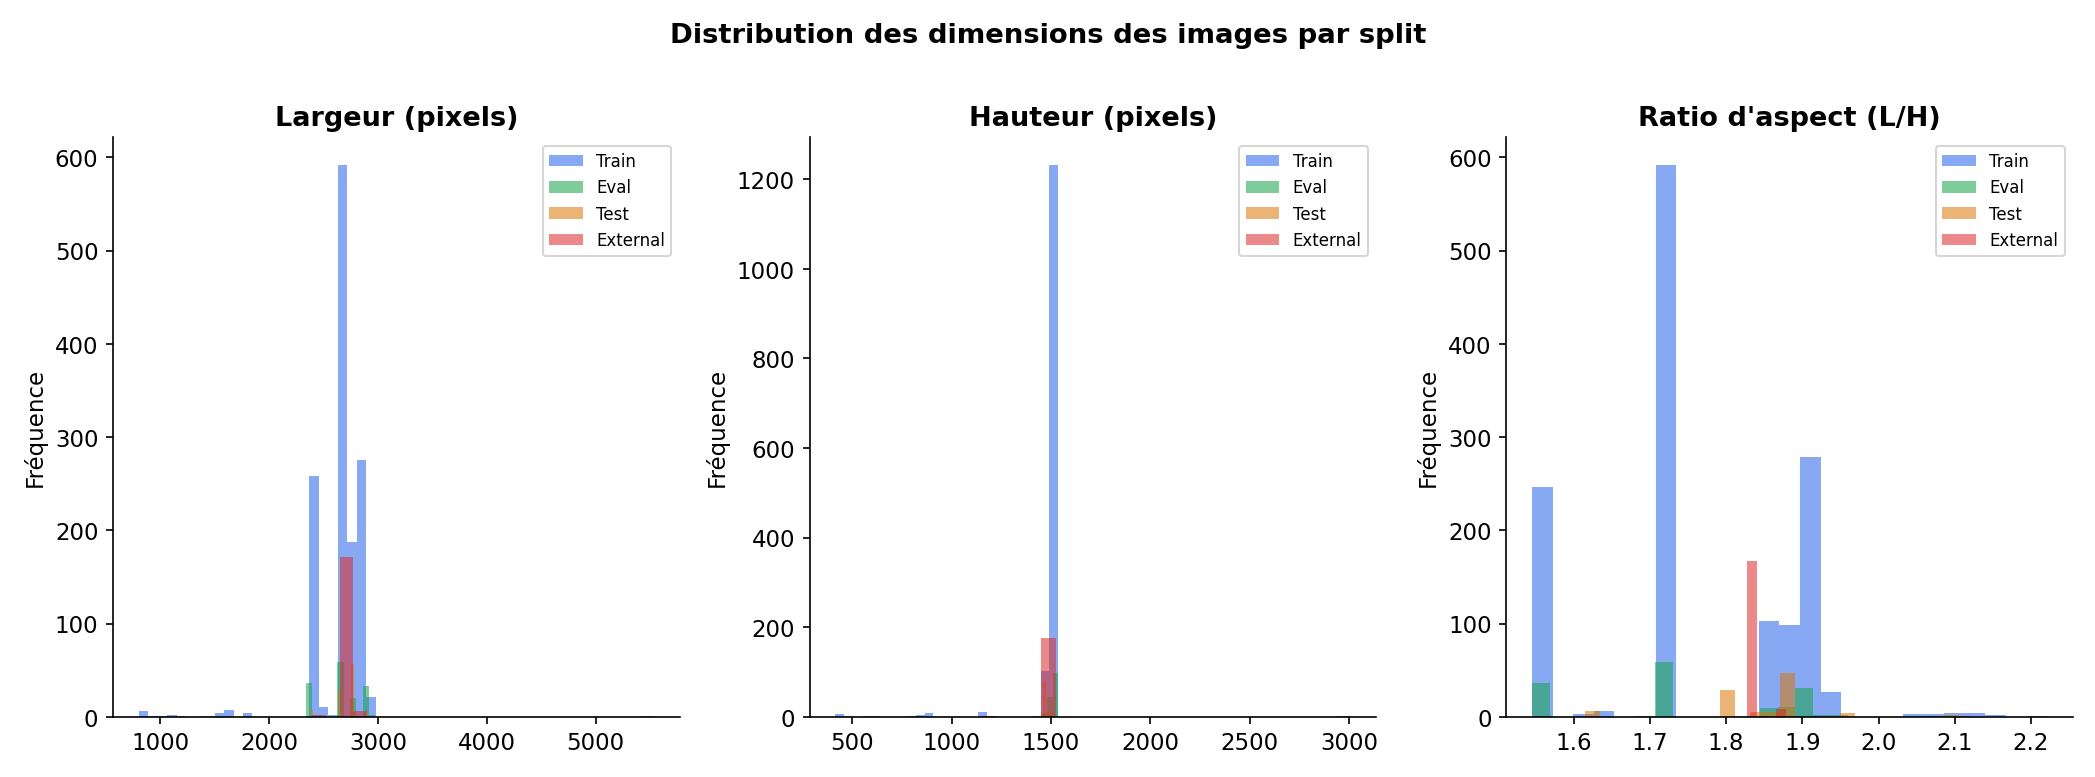
\includegraphics[width=\textwidth]{figures/eda_image_dimensions.png}
\caption{Distribution des largeurs, hauteurs et ratios d'aspect des images par partition}
\label{fig:img_dims}
\end{figure}

La figure~\ref{fig:img_dims} révèle une homogénéité satisfaisante des dimensions
au sein du corpus. Les résolutions dominantes par partition sont :

\begin{table}[H]
\centering
\caption{Résolutions dominantes et statistiques des images par partition}
\label{tab:image_sizes}
\begin{tabular}{lllr}
\toprule
\textbf{Partition} & \textbf{Résolution dominante} & \textbf{Médiane approx.}
                   & \textbf{Couverture} \\
\midrule
train    & $2\,652 \times 1\,536$ px & $2\,652 \times 1\,536$ px & 34.5\% \\
eval     & $2\,652 \times 1\,536$ px & $2\,652 \times 1\,536$ px & 28.8\% \\
test     & $2\,775 \times 1\,475$ px & $2\,775 \times 1\,475$ px & 46.0\% \\
external & $2\,760 \times 1\,504$ px & $2\,760 \times 1\,504$ px & 92.2\% \\
\bottomrule
\end{tabular}
\end{table}

Le ratio d'aspect moyen est stable autour de $\approx 1.75$ pour toutes les
partitions, cohérent avec la géométrie caractéristique des orthopantomogrammes.
Cette homogénéité est favorable à l'entraînement d'un détecteur unique sans
adaptation spécifique par partition.

\subsection{Images Atypiques dans le Split Train}

Le split \texttt{train} contient quelques images à résolutions atypiques :
6 images à $804 \times 415$ px, 1 image à $938 \times 491$ px et plusieurs
images autour de $1\,600 \times 870$ px. Ces images, nettement plus petites
que la résolution standard, proviennent probablement de sources d'acquisition
différentes ou ont été recadrées. Leur présence dans le corpus d'entraînement
peut contribuer positivement à la robustesse du modèle face à la variabilité
de résolution.

\section{Analyse des Annotations}

\subsection{Volumes par Partition}

\begin{table}[H]
\centering
\caption{Statistiques des annotations par partition (dataset brut)}
\label{tab:annotations_stats}
\begin{tabular}{lrrrr}
\toprule
\textbf{Partition} & \textbf{Images} & \textbf{Objets} & \textbf{Obj./image}
                   & \textbf{Labels invalides} \\
\midrule
train    & 1\,375 & 18\,570 & 13.50 & 2 \\
eval     & 153    & 1\,972  & 12.89 & 0 \\
test     & 100    & 1\,369  & 13.69 & 0 \\
external & 180    & 2\,980  & 16.55 & 1 \\
\midrule
\textbf{Total} & \textbf{1\,808} & \textbf{24\,891} & \textbf{13.76} & \textbf{3} \\
\bottomrule
\end{tabular}
\end{table}

\begin{figure}[H]
\centering
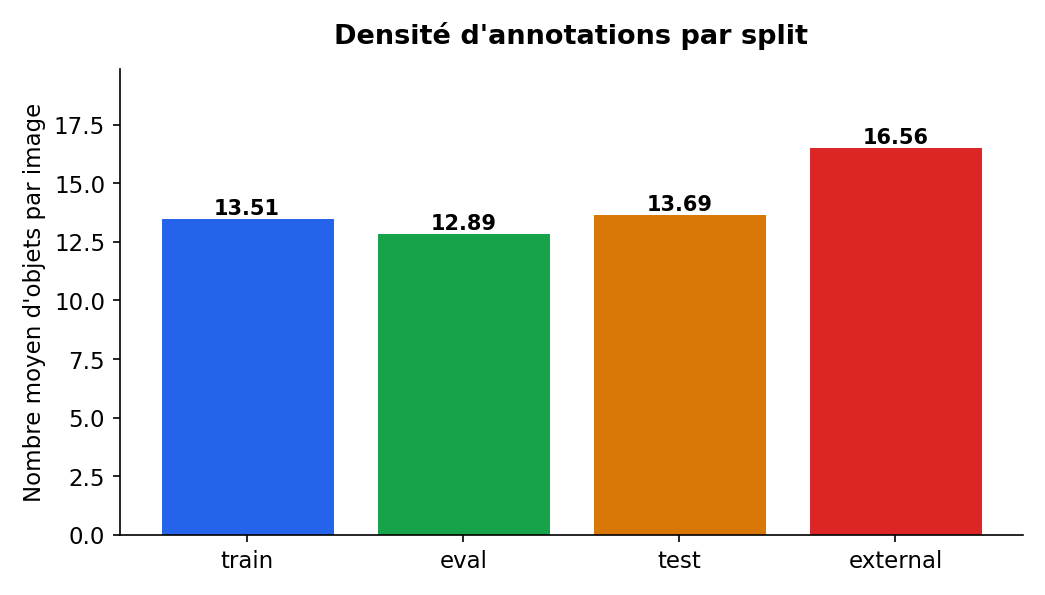
\includegraphics[width=0.72\textwidth]{figures/eda_objects_per_image.png}
\caption{Nombre moyen d'objets annotés par image, par partition}
\label{fig:obj_density}
\end{figure}

La figure~\ref{fig:obj_density} met en évidence que la partition \texttt{external}
présente une densité d'annotations significativement plus élevée que les autres
partitions : \textbf{16.55 objets par image} contre 13.50 pour \texttt{train}.
Cette densité plus importante suggère que les praticiens du cabinet externe
annotaient plus systématiquement l'ensemble des structures visibles, ou que
leur patientèle présente davantage de pathologies simultanées. Dans les deux cas,
cela constitue un défi supplémentaire pour le modèle lors de l'évaluation sur ce split.

\section{Taxonomie des 14 Classes Originales}

\subsection{Description des Classes}

Le dataset brut comporte 14 classes d'annotation couvrant l'ensemble des
structures et pathologies visibles sur une radiographie panoramique.

\begin{table}[H]
\centering
\caption{Distribution des 14 classes originales — tous splits confondus}
\label{tab:14_classes_distribution}
\begin{tabular}{clrrl}
\toprule
\textbf{ID} & \textbf{Classe} & \textbf{Total} & \textbf{\%} & \textbf{Images} \\
\midrule
2  & Obturation              & 5\,262 & 21.5\% & 1\,027 \\
5  & Bone resorption         & 3\,858 & 15.8\% & 588    \\
3  & Endodontic treatment    & 3\,692 & 15.1\% & 1\,048 \\
4  & Carious lesion          & 3\,589 & 14.7\% & 1\,068 \\
1  & Prosthetic restoration  & 1\,890 & 7.7\%  & 711    \\
8  & Root fragment           & 1\,502 & 6.1\%  & 505    \\
13 & Surgical device         & 1\,272 & 5.2\%  & 252    \\
7  & Apical periodontitis    & 1\,259 & 5.1\%  & 654    \\
6  & Impacted tooth          & 1\,088 & 4.4\%  & 448    \\
12 & Orthodontic device      & 533    & 2.2\%  & 232    \\
0  & Implant                 & 522    & 2.1\%  & 152    \\
9  & Furcation lesion        & 328    & 1.3\%  & 226    \\
10 & Apical surgery          & 91     & 0.4\%  & 51     \\
11 & Root resorption         & 5      & 0.0\%  & 4      \\
\midrule
   & \textbf{Total}          & \textbf{24\,891} & \textbf{100\%} & -- \\
\bottomrule
\end{tabular}
\end{table}

\begin{figure}[H]
\centering
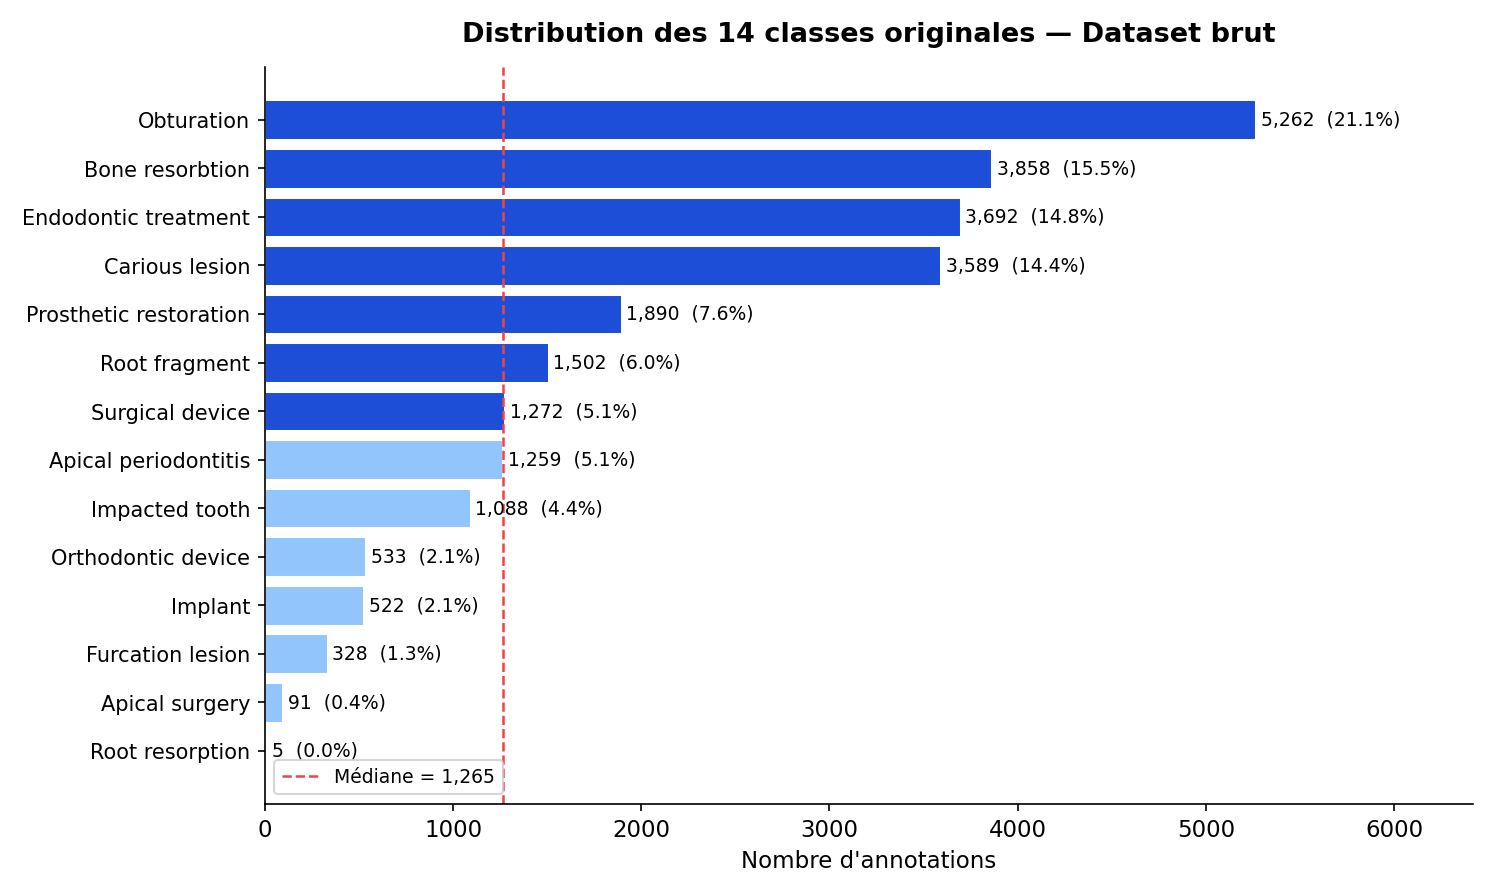
\includegraphics[width=0.95\textwidth]{figures/eda_raw_class_distribution.png}
\caption{Distribution des 14 classes originales dans le dataset brut (tous splits confondus)}
\label{fig:raw_class_dist}
\end{figure}

\subsection{Problèmes Identifiés dans la Taxonomie}

L'analyse de la figure~\ref{fig:raw_class_dist} et du
tableau~\ref{tab:14_classes_distribution} révèle trois catégories de problèmes.

\textbf{Déséquilibre sévère.} Les 4 classes les plus fréquentes
(\textit{Obturation}, \textit{Bone resorption}, \textit{Endodontic treatment},
\textit{Carious lesion}) concentrent \textbf{67.1\%} des annotations totales.
À l'opposé, \textit{Root resorption} (5 objets, 0.02\%) et
\textit{Apical surgery} (91 objets, 0.37\%) sont statistiquement inexploitables
en apprentissage individuel.

\textbf{Redondance sémantique.} Plusieurs classes désignent des états
cliniquement proches qui pourraient être regroupés sans perte d'information
diagnostique : \textit{Obturation}, \textit{Endodontic treatment},
\textit{Prosthetic restoration} et \textit{Apical surgery} désignent toutes
des dents ayant reçu un traitement. De même, \textit{Implant},
\textit{Orthodontic device} et \textit{Surgical device} sont tous des dispositifs
artificiels visibles sur le cliché.

\textbf{Absence dans certains splits.} La classe \textit{Root resorption} est
totalement absente des splits \texttt{eval}, \texttt{test} et \texttt{external}
(0 annotation dans chacun). Son apprentissage est donc basé uniquement sur 5
exemples de \texttt{train}, ce qui la rend inutilisable comme classe indépendante.

Ces trois problèmes motivent directement le remappage vers 7 classes présenté
au Chapitre~\ref{chap:data_preparation}.

\section{Distribution des 7 Classes Après Remappage}

\subsection{Volumes Globaux}

\begin{figure}[H]
\centering
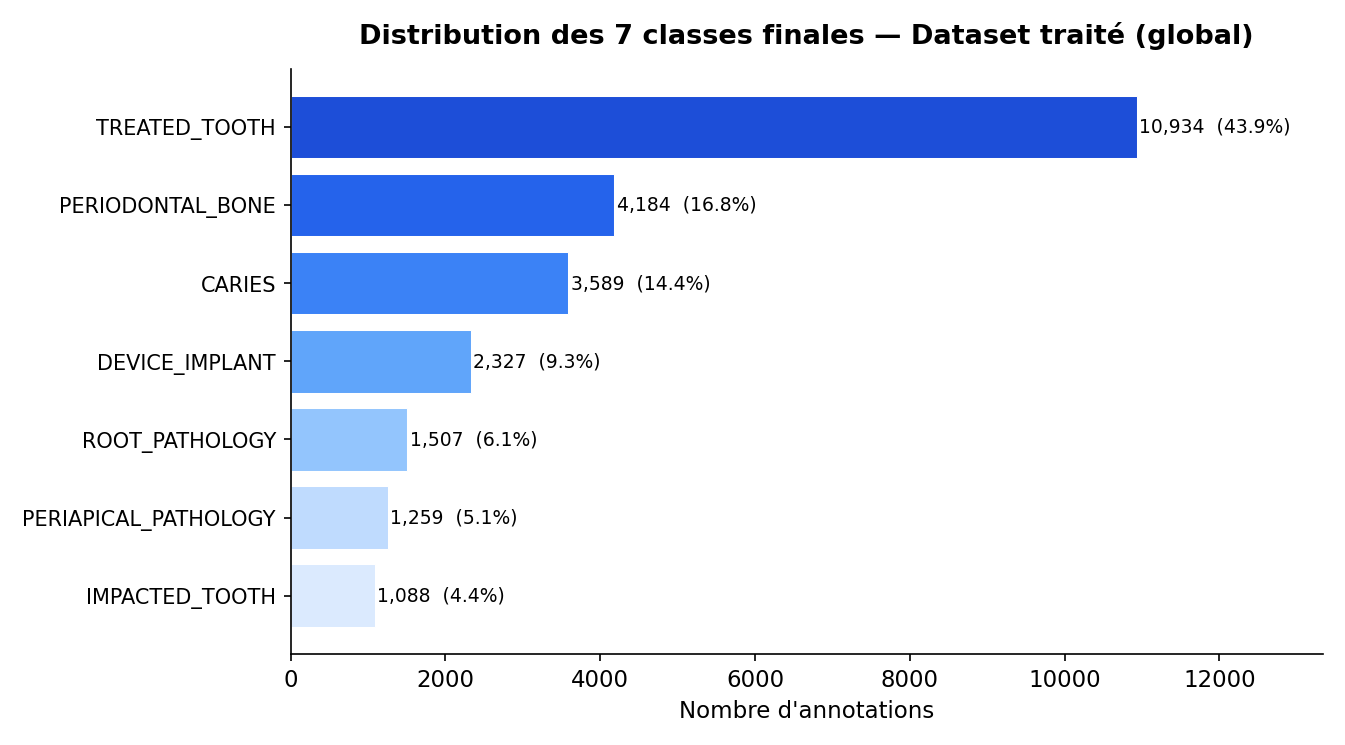
\includegraphics[width=0.92\textwidth]{figures/eda_processed_class_distribution.png}
\caption{Distribution des 7 classes finales dans le dataset traité (tous splits confondus)}
\label{fig:processed_class_dist}
\end{figure}

\begin{table}[H]
\centering
\caption{Distribution des 7 classes finales — dataset traité, tous splits confondus}
\label{tab:7_classes_global}
\begin{tabular}{clrrl}
\toprule
\textbf{ID} & \textbf{Classe} & \textbf{Total} & \textbf{\%} & \textbf{Images} \\
\midrule
5 & \texttt{TREATED\_TOOTH}        & 10\,934 & 43.9\% & 1\,355 \\
2 & \texttt{PERIODONTAL\_BONE}      & 4\,184  & 16.8\% & 685    \\
0 & \texttt{CARIES}                 & 3\,589  & 14.4\% & 1\,068 \\
6 & \texttt{DEVICE\_IMPLANT}        & 2\,327  & 9.3\%  & 447    \\
4 & \texttt{ROOT\_PATHOLOGY}        & 1\,507  & 6.1\%  & 509    \\
1 & \texttt{PERIAPICAL\_PATHOLOGY}  & 1\,259  & 5.1\%  & 654    \\
3 & \texttt{IMPACTED\_TOOTH}        & 1\,088  & 4.4\%  & 448    \\
\midrule
  & \textbf{Total}                  & \textbf{24\,888} & \textbf{100\%} & -- \\
\bottomrule
\end{tabular}
\end{table}

Après remappage, \texttt{TREATED\_TOOTH} devient la classe dominante avec
\textbf{10\,934 objets (43.9\%}), résultat du regroupement de 4 classes originales
(Obturation, Prosthetic restoration, Endodontic treatment, Apical surgery).
Toutes les 7 classes disposent désormais d'au moins 1\,000 exemples dans le
corpus global, rendant leur apprentissage statistiquement viable.

\subsection{Distribution par Partition}

\begin{figure}[H]
\centering
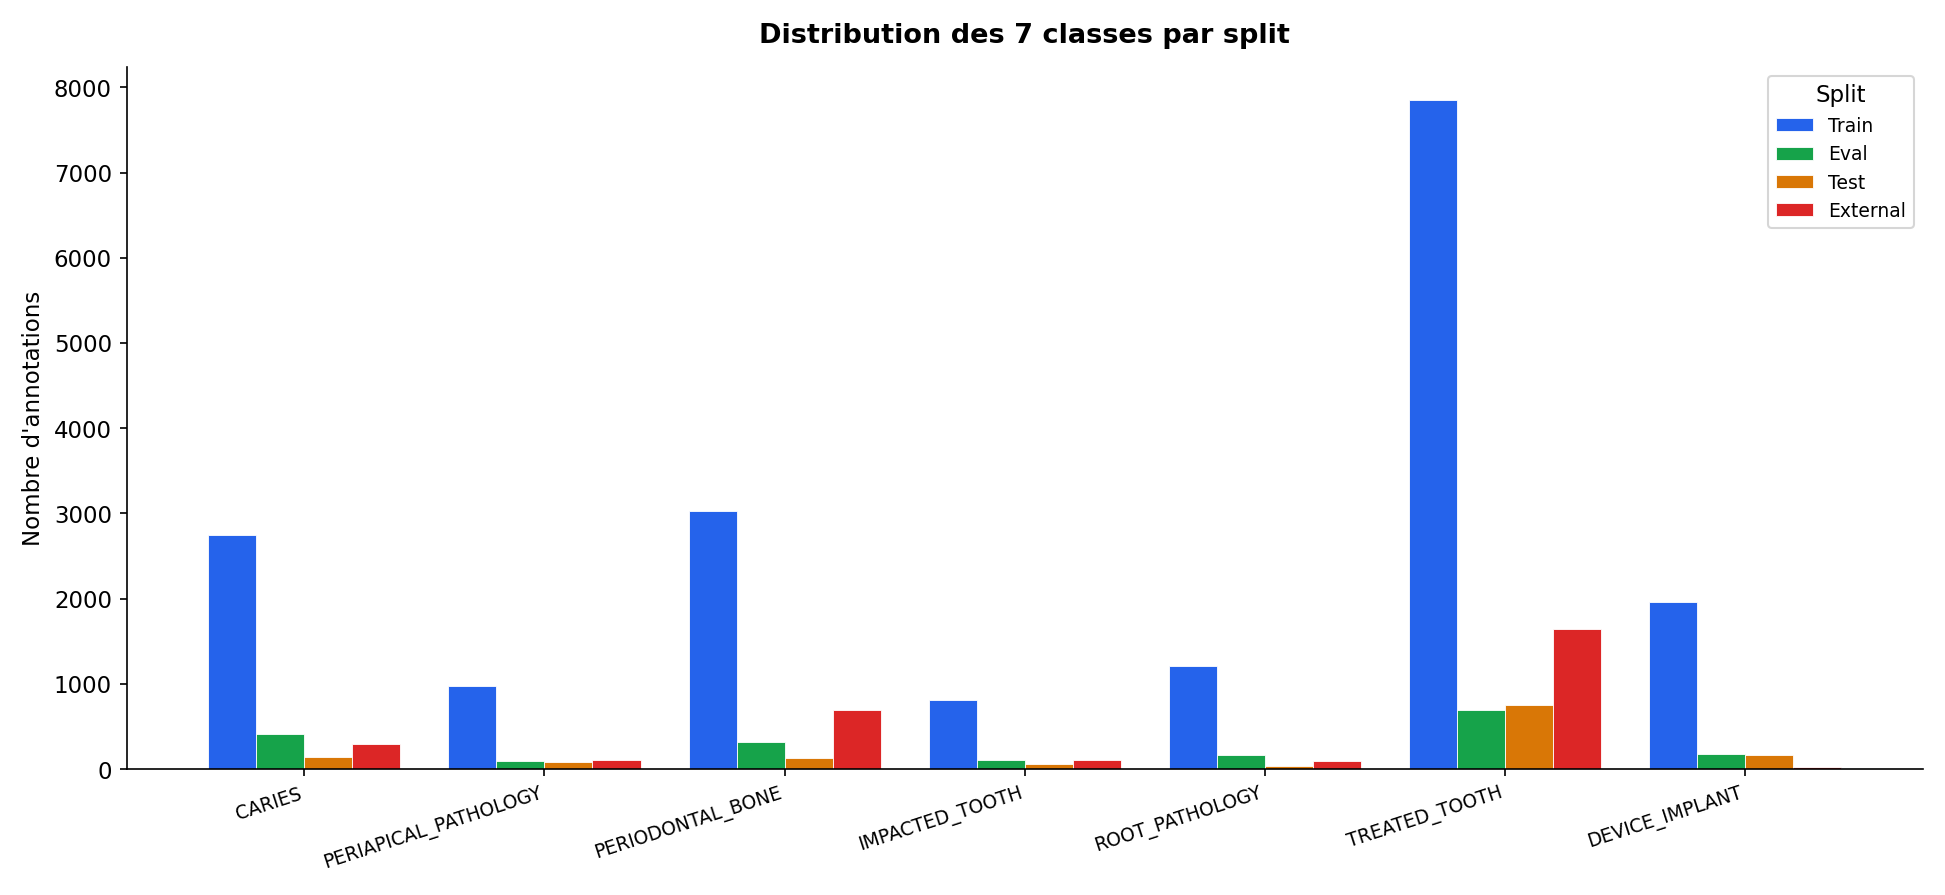
\includegraphics[width=\textwidth]{figures/eda_class_distribution_per_split.png}
\caption{Distribution des 7 classes finales par partition}
\label{fig:class_per_split}
\end{figure}

\begin{figure}[H]
\centering
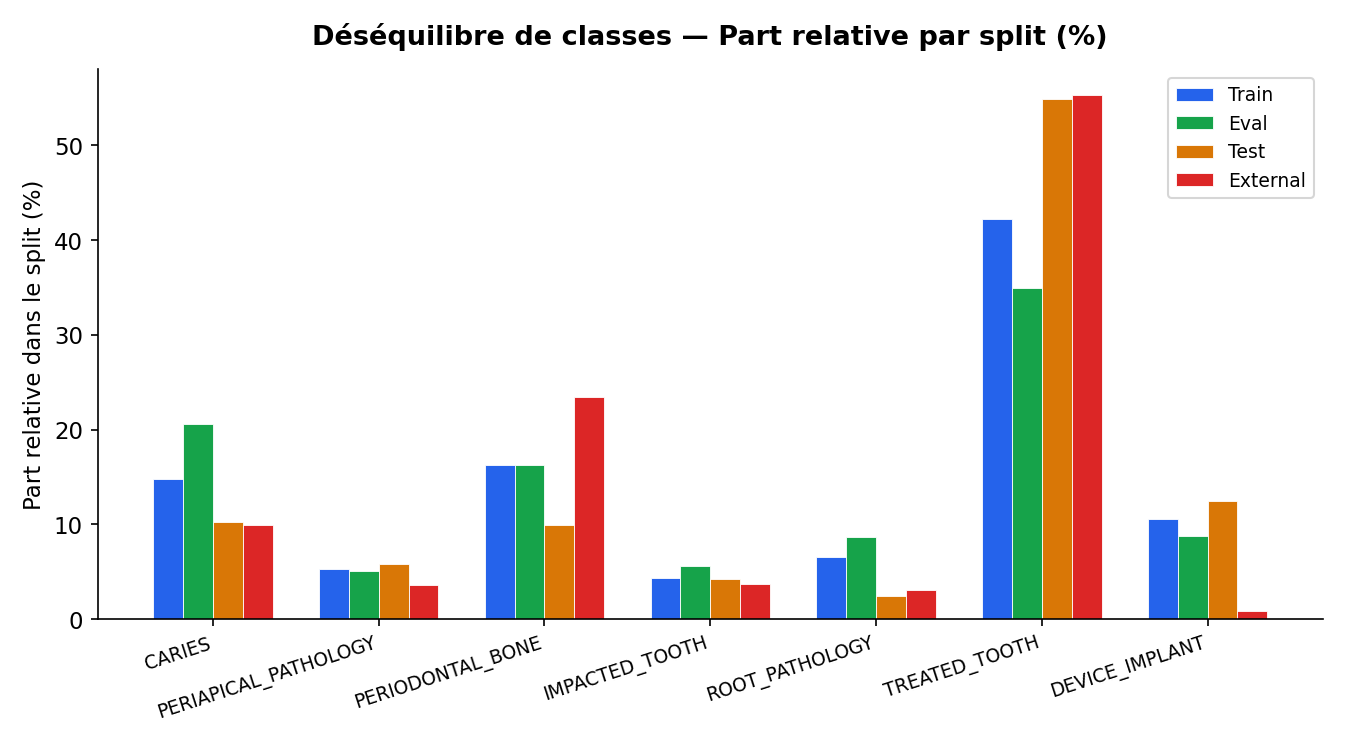
\includegraphics[width=\textwidth]{figures/eda_class_imbalance_pct.png}
\caption{Part relative (\%) de chaque classe par partition — mise en évidence du déséquilibre inter-splits}
\label{fig:imbalance_pct}
\end{figure}

\begin{table}[H]
\centering
\caption{Distribution détaillée des 7 classes par partition (dataset traité)}
\label{tab:7_classes_per_split}
\begin{tabular}{lrrrrr}
\toprule
\textbf{Classe} & \textbf{train} & \textbf{eval} & \textbf{test}
                & \textbf{external} & \textbf{Total} \\
\midrule
\texttt{TREATED\_TOOTH}       & 7\,846 & 690 & 751   & 1\,647 & 10\,934 \\
\texttt{PERIODONTAL\_BONE}    & 3\,029 & 320 & 136   & 699    & 4\,184  \\
\texttt{CARIES}               & 2\,745 & 407 & 141   & 296    & 3\,589  \\
\texttt{DEVICE\_IMPLANT}      & 1\,956 & 174 & 170   & 27     & 2\,327  \\
\texttt{ROOT\_PATHOLOGY}      & 1\,210 & 171 & 33    & 93     & 1\,507  \\
\texttt{PERIAPICAL\_PATHOLOGY}& 973    & 100 & 80    & 106    & 1\,259  \\
\texttt{IMPACTED\_TOOTH}      & 809    & 110 & 58    & 111    & 1\,088  \\
\midrule
\textbf{Total}                & \textbf{18\,568} & \textbf{1\,972}
                              & \textbf{1\,369}  & \textbf{2\,979}
                              & \textbf{24\,888} \\
\bottomrule
\end{tabular}
\end{table}

L'analyse croisée des figures~\ref{fig:class_per_split} et~\ref{fig:imbalance_pct}
et du tableau~\ref{tab:7_classes_per_split} met en évidence deux observations
importantes concernant la partition \texttt{external}.

Premièrement, \texttt{DEVICE\_IMPLANT} est quasi absente dans \texttt{external}
avec seulement \textbf{27 objets} contre 170 dans \texttt{test} et 174 dans
\texttt{eval}. Cela reflète probablement une pratique clinique différente du
cabinet externe, avec moins d'implants et de dispositifs orthodontiques dans
leur patientèle.

Deuxièmement, \texttt{PERIODONTAL\_BONE} est sur-représentée dans
\texttt{external} avec \textbf{699 objets} (23.5\% du split) contre 16.2\%
dans \texttt{eval} et seulement 9.9\% dans \texttt{test}. Cette différence
de distribution constitue un défi de généralisation que le modèle devra surmonter.


\section{Conclusion}

Cette phase de compréhension des données a permis d'établir une connaissance
approfondie et chiffrée du corpus. Le dataset est structurellement sain —
0 image corrompue, 0 label manquant, 0 doublon — avec seulement 3 annotations
invalides sur 24\,891 (0.012\%). La taxonomie originale de 14 classes présente
des déséquilibres sévères et des redondances sémantiques qui motivent un
remappage vers 7 classes cliniques plus robustes. La partition \texttt{external}
présente des caractéristiques de distribution distinctes qui en font un
indicateur de généralisation exigeant et réaliste. Toutes ces observations
ont directement alimenté les décisions de préparation des données présentées
dans le chapitre suivant.



\chapter{Préparation des Données}
\label{chap:data_preparation}

\section{Introduction}

La troisième phase de CRISP-DM, la préparation des données (\textit{Data Preparation}),
couvre l'ensemble des opérations nécessaires pour transformer les données brutes
en un corpus exploitable par les algorithmes de modélisation. Dans ce projet,
cette phase est particulièrement structurante car elle ne se limite pas à un
simple nettoyage : elle implique une restructuration complète de la taxonomie
des classes, une validation ligne par ligne des annotations, un versionnement
rigoureux des artéfacts et une conception orientée reproductibilité. Toutes ces
opérations sont formalisées dans un pipeline DVC reproductible, ce qui constitue
l'une des contributions MLOps essentielles du projet.

\section{Architecture du Pipeline de Données avec DVC}

\subsection{Pourquoi DVC ?}

DVC (\textit{Data Version Control}) est un outil open-source conçu pour étendre
les capacités de Git aux données volumineuses et aux pipelines ML~\cite{dvc2020}.
Il résout un problème fondamental du MLOps : Git gère bien le code, mais pas les
fichiers de données volumineux ni les artéfacts binaires (modèles, datasets).
DVC permet de :

\begin{itemize}
    \item \textbf{versionner les données} sans les stocker dans Git, en utilisant
          des fichiers \texttt{.dvc} comme pointeurs vers un stockage externe ou local ;
    \item \textbf{définir des pipelines reproductibles} avec des dépendances
          explicites entre les étapes (entrées, sorties, commandes) ;
    \item \textbf{détecter automatiquement} quelles étapes doivent être réexécutées
          lorsque les données ou le code changent (\texttt{dvc repro}) ;
    \item \textbf{tracer} l'ensemble des transformations appliquées aux données,
          garantissant la reproductibilité bout en bout.
\end{itemize}

\subsection{Structure du Pipeline DVC}

Le pipeline DVC du projet est défini dans \projectpath{dvc.yaml} et comporte
trois stages séquentiels, chacun ayant des dépendances et des sorties explicitement
déclarées.

\begin{figure}[H]
\centering
\fbox{\begin{minipage}[c][0.12\textheight][c]{0.75\linewidth}
\centering
\Large
\texttt{inspect} $\longrightarrow$ \texttt{prepare} $\longrightarrow$ \texttt{stats}\\[0.8em]
\normalsize
\textit{data/raw/} \hspace{1.2cm} \textit{data/processed/} \hspace{0.8cm}
\textit{reports/tables/}
\end{minipage}}
\caption{Enchaînement des stages du pipeline DVC}
\label{fig:dvc_pipeline}
\end{figure}


\subsection{Reproductibilité par \texttt{dvc repro}}

La commande \texttt{dvc repro} analyse le graphe de dépendances du pipeline et
réexécute uniquement les stages dont les entrées ont changé. Ce mécanisme garantit
que :

\begin{itemize}
    \item toute modification du code de préparation déclenche automatiquement
          la régénération du dataset traité ;
    \item toute modification du dataset brut propage automatiquement les changements
          vers les statistiques finales ;
    \item un collaborateur qui clone le dépôt peut reproduire exactement le même
          dataset traité en une seule commande.
\end{itemize}

\section{Stage 1 : Audit du Dataset Brut (\texttt{inspect})}

\subsection{Objectif et Implémentation}

Le stage \texttt{inspect} exécute le script \projectpath{scripts/inspect\_dataset.py}.
Ce script parcourt le dataset brut et vérifie systématiquement pour chaque partition :
la cohérence image-label, l'intégrité des fichiers images, la validité géométrique
des annotations YOLO et l'absence de doublons. Les résultats sont persistés dans
\projectpath{reports/summaries/inspect\_report.json}.

\subsection{Résultats de l'Audit sur le Dataset Brut}

\begin{table}[H]
\centering
\caption{Résultats comparatifs de la vérification des labels — brut vs traité}
\label{tab:verify_comparison}
\begin{tabular}{lrrrr}
\toprule
\textbf{Partition} & \multicolumn{2}{c}{\textbf{Dataset brut}}
                   & \multicolumn{2}{c}{\textbf{Dataset traité}} \\
\cmidrule(lr){2-3} \cmidrule(lr){4-5}
                   & \textbf{Objets} & \textbf{Invalides}
                   & \textbf{Objets} & \textbf{Invalides} \\
\midrule
train    & 18\,570 & 2 & 18\,568 & 0 \\
eval     & 1\,972  & 0 & 1\,972  & 0 \\
test     & 1\,369  & 0 & 1\,369  & 0 \\
external & 2\,980  & 1 & 2\,979  & 0 \\
\midrule
\textbf{Total} & \textbf{24\,891} & \textbf{3} & \textbf{24\,888} & \textbf{0} \\
\bottomrule
\end{tabular}
\end{table}

Ce tableau démontre l'efficacité du pipeline de préparation : les 3 annotations
invalides du dataset brut (fichiers \texttt{56.txt}, \texttt{97.txt} et
\texttt{128.txt}) ont été intégralement filtrées. Le dataset traité présente
\textbf{0 label invalide} sur l'ensemble des 1\,808 fichiers de labels,
confirmant la robustesse du mécanisme de validation.

\section{Stage 2 : Préparation du Dataset 7 Classes (\texttt{prepare})}

\subsection{Vue d'Ensemble du Script}

Le stage \texttt{prepare} constitue le cœur du pipeline de données. Il est
implémenté dans \projectpath{scripts/prepare\_dataset\_7classes.py} et
s'appuie sur les modules du package \projectpath{src/detection\_dentaire/data/}.
Ce script réalise les opérations suivantes dans l'ordre :

\begin{enumerate}
    \item \textbf{Détection automatique des splits} : le script identifie les
          dossiers \texttt{train}, \texttt{valid}, \texttt{test} et
          \texttt{test\_alte\_cabinete/Ext-validation} dans le dataset brut.
    \item \textbf{Renommage des splits} : le split \texttt{valid} est renommé
          \texttt{eval} dans le dataset traité pour lever l'ambiguïté avec la
          validation interne d'Ultralytics.
    \item \textbf{Copie des images} : chaque image est copiée vers la structure
          cible (option \texttt{--copy-images}).
    \item \textbf{Traitement des labels} : chaque fichier de labels est relu,
          validé ligne par ligne, remappe et réécrit.
    \item \textbf{Génération des fichiers de documentation} : YAML dataset,
          fichier de mapping, résumé JSON.
\end{enumerate}

\subsection{Implémentation du Remappage 14 $\rightarrow$ 7 Classes}

Le remappage est implémenté dans le module
\projectpath{src/detection\_dentaire/data/remap.py}.
La logique centrale repose sur un dictionnaire de correspondance statique qui
associe chaque identifiant de classe original à son identifiant de classe cible.

\begin{table}[H]
\centering
\caption{Table de remappage complète : 14 classes originales $\rightarrow$ 7 classes finales}
\label{tab:remap_complet}
\begin{tabular}{clcl}
\toprule
\textbf{ID original} & \textbf{Classe originale} & \textbf{ID final} & \textbf{Classe finale} \\
\midrule
4  & Carious lesion          & 0 & \texttt{CARIES} \\
\midrule
7  & Apical periodontitis    & 1 & \texttt{PERIAPICAL\_PATHOLOGY} \\
\midrule
5  & Bone resorption         & 2 & \texttt{PERIODONTAL\_BONE} \\
9  & Furcation lesion        & 2 & \texttt{PERIODONTAL\_BONE} \\
\midrule
6  & Impacted tooth          & 3 & \texttt{IMPACTED\_TOOTH} \\
\midrule
8  & Root fragment           & 4 & \texttt{ROOT\_PATHOLOGY} \\
11 & Root resorption         & 4 & \texttt{ROOT\_PATHOLOGY} \\
\midrule
1  & Prosthetic restoration  & 5 & \texttt{TREATED\_TOOTH} \\
2  & Obturation              & 5 & \texttt{TREATED\_TOOTH} \\
3  & Endodontic treatment    & 5 & \texttt{TREATED\_TOOTH} \\
10 & Apical surgery          & 5 & \texttt{TREATED\_TOOTH} \\
\midrule
0  & Implant                 & 6 & \texttt{DEVICE\_IMPLANT} \\
12 & Orthodontic device      & 6 & \texttt{DEVICE\_IMPLANT} \\
13 & Surgical device         & 6 & \texttt{DEVICE\_IMPLANT} \\
\bottomrule
\end{tabular}
\end{table}

La fonction \texttt{remap\_records()} du module prend en entrée une liste de
tuples \texttt{(class\_id, x\_center, y\_center, width, height)} et retourne
la même liste avec les identifiants de classes remappés. Les coordonnées
géométriques des boîtes englobantes sont conservées à l'identique — seul
l'identifiant de classe est modifié.

\subsection{Validation Ligne par Ligne des Labels}

Avant d'appliquer le remappage, chaque ligne de chaque fichier de labels
est validée par la fonction \texttt{validate\_yolo\_record()} du module
\projectpath{src/detection\_dentaire/data/}. Les vérifications appliquées sont :

\begin{itemize}
    \item présence exacte de 5 valeurs numériques par ligne ;
    \item identifiant de classe appartenant à l'ensemble des 14 classes autorisées
          $\{0, \ldots, 13\}$ ;
    \item coordonnées $x_c, y_c, w, h$ dans l'intervalle $]0, 1]$ ;
    \item dimensions $w > 0$ et $h > 0$ (filtre les annotations dégénérées).
\end{itemize}

Toute ligne ne passant pas ces vérifications est ignorée et comptabilisée dans
les statistiques de préparation, sans interrompre le traitement de l'ensemble
du fichier. Ce comportement garantit la robustesse du pipeline face aux
annotations corrompues.

\subsection{Structure du Dataset Traité}

Le dataset traité généré dans \projectpath{data/processed/dataset\_7classes/}
adopte la structure suivante :

\begin{figure}[H]
\centering
\fbox{\begin{minipage}{0.75\linewidth}
\ttfamily\small
dataset\_7classes/\\
\hspace*{1em}├── train/\\
\hspace*{2em}│\hspace*{1em}├── images/ \hfill (1\,375 images)\\
\hspace*{2em}│\hspace*{1em}└── labels/ \hfill (1\,375 fichiers)\\
\hspace*{1em}├── eval/\\
\hspace*{2em}│\hspace*{1em}├── images/ \hfill (153 images)\\
\hspace*{2em}│\hspace*{1em}└── labels/ \hfill (153 fichiers)\\
\hspace*{1em}├── test/\\
\hspace*{2em}│\hspace*{1em}├── images/ \hfill (100 images)\\
\hspace*{2em}│\hspace*{1em}└── labels/ \hfill (100 fichiers)\\
\hspace*{1em}├── test\_alte\_cabinete/Ext-validation/\\
\hspace*{2em}│\hspace*{1em}├── images/ \hfill (180 images)\\
\hspace*{2em}│\hspace*{1em}└── labels/ \hfill (180 fichiers)\\
\hspace*{1em}├── data\_7classes.yaml\\
\hspace*{1em}├── class\_mapping\_14\_to\_7.json\\
\hspace*{1em}├── labels\_7classes.txt\\
\hspace*{1em}└── prepare\_summary.json
\end{minipage}}
\caption{Structure du dataset traité \texttt{dataset\_7classes/}}
\label{fig:dataset_structure}
\end{figure}

\subsection{Fichiers de Documentation Générés}

Le script génère automatiquement quatre fichiers de documentation :

\begin{table}[H]
\centering
\caption{Fichiers de documentation générés par le pipeline de préparation}
\label{tab:fichiers_doc}
\begin{tabular}{p{5.5cm} p{8.5cm}}
\toprule
\textbf{Fichier} & \textbf{Contenu} \\
\midrule
\texttt{data\_7classes.yaml}
  & Configuration YAML au format Ultralytics décrivant les chemins des splits
    et les 7 classes cibles. Utilisé directement par YOLOv8 lors de l'entraînement. \\
\midrule
\texttt{class\_mapping\_14\_to\_7.json}
  & Dictionnaire JSON contenant les noms des 14 classes originales, les 7 classes
    finales et la table de correspondance complète. Permet de tracer les décisions
    de remappage. \\
\midrule
\texttt{labels\_7classes.txt}
  & Fichier texte listant les 7 noms de classes, un par ligne. Compatible avec les
    outils de visualisation d'annotations. \\
\midrule
\texttt{prepare\_summary.json}
  & Résumé détaillé de la préparation par split : nombre d'images, d'objets,
    de labels invalides filtrés, comptages par classe avant et après remappage. \\
\bottomrule
\end{tabular}
\end{table}

\section{Stage 3 : Calcul des Statistiques (\texttt{stats})}

Le stage \texttt{stats} exécute \projectpath{scripts/class\_stats.py} sur le
dataset traité. Il calcule pour chaque partition et pour le corpus global :
le nombre d'objets par classe, le nombre d'images contenant chaque classe,
et les totaux agrégés. Les résultats sont exportés simultanément en
\texttt{CSV} (\projectpath{reports/tables/class\_stats.csv}) pour une
consultation tabulaire et en \texttt{JSON}
(\projectpath{reports/summaries/class\_stats.json}) pour une exploitation
programmatique. Ces statistiques alimentent directement les figures EDA
du Chapitre~\ref{chap:data_understanding} et les décisions de configuration
de l'entraînement du Chapitre~\ref{chap:modeling}.

\section{Vérification du Dataset Traité}

\subsection{Audit Post-Préparation}

Après la génération du dataset traité, un second audit a été conduit via
\projectpath{scripts/inspect\_dataset.py} sur
\projectpath{data/processed/dataset\_7classes/}, dont les résultats sont
dans
\projectpath{reports/summaries/inspect\_processed.json}.

\begin{table}[H]
\centering
\caption{Résultats de l'audit du dataset traité — tous splits}
\label{tab:audit_processed}
\begin{tabular}{lcccccc}
\toprule
\textbf{Split} & \textbf{Images} & \textbf{Labels} & \textbf{Manquants}
               & \textbf{Orphelins} & \textbf{Corrompus} & \textbf{Invalides} \\
\midrule
train    & 1\,375 & 1\,375 & 0 & 0 & 0 & \textbf{0} \\
eval     & 153    & 153    & 0 & 0 & 0 & \textbf{0} \\
test     & 100    & 100    & 0 & 0 & 0 & \textbf{0} \\
external & 180    & 180    & 0 & 0 & 0 & \textbf{0} \\
\midrule
\textbf{Total} & \textbf{1\,808} & \textbf{1\,808} & \textbf{0} & \textbf{0}
               & \textbf{0} & \textbf{0} \\
\bottomrule
\end{tabular}
\end{table}

Le dataset traité est \textbf{structurellement parfait} : aucune anomalie
détectée sur l'ensemble des 1\,808 images et 1\,808 fichiers de labels.
Ce résultat confirme que le pipeline de préparation a correctement filtré
les 3 annotations invalides du dataset brut et produit un corpus entièrement
sain pour l'entraînement et l'évaluation.

\subsection{Vérification des Labels Traités}

Un second outil de vérification, \projectpath{scripts/verify\_yolo\_labels.py},
a validé la cohérence des labels du dataset traité avec les 7 classes attendues.
Les résultats, dans \projectpath{reports/summaries/verify\_processed\_labels.json},
confirment :

\begin{itemize}
    \item \textbf{0 fichier de label invalide} sur les 1\,808 fichiers vérifiés ;
    \item \textbf{0 fichier de label vide} ;
    \item \textbf{24\,888 objets valides} au total,
          tous avec des identifiants de classe dans $\{0, \ldots, 6\}$.
\end{itemize}

\section{Garanties de Reproductibilité}

La reproductibilité du pipeline de données repose sur cinq mécanismes complémentaires.

\textbf{Versionnage DVC.} Le dataset brut est référencé par le fichier
\projectpath{data/raw/dataset\_original.dvc} qui contient le hash MD5 du
répertoire. Toute modification du dataset brut est détectée par DVC qui
invalidera automatiquement les stages en aval.

\textbf{Seed globale.} La variable \texttt{project.seed = 42} dans
\projectpath{params.yaml} est utilisée par tous les scripts pour garantir
la reproductibilité des opérations aléatoires.

\textbf{Configuration externalisée.} Tous les paramètres (chemins, classes,
splits) sont centralisés dans \projectpath{params.yaml} et
\projectpath{configs/data.yaml}. Aucun paramètre n'est codé en dur dans
les scripts.

\textbf{Idempotence.} Le script \texttt{prepare\_dataset\_7classes.py} est
conçu pour être idempotent : il réinitialise le répertoire destination avant
chaque exécution (\texttt{reset\_dir()}), garantissant que deux exécutions
successives produisent exactement le même résultat.

\textbf{Traçabilité des artéfacts.} Chaque exécution du pipeline génère
\texttt{prepare\_summary.json} qui documente précisément les transformations
appliquées, les labels filtrés et les comptages par classe, constituant une
piste d'audit complète de la préparation des données.

\section{Conclusion}

Ce chapitre a présenté le pipeline de préparation des données du projet,
articulé en trois stages DVC reproductibles. Le résultat central est la
transformation d'un corpus brut de 24\,891 annotations sur 14 classes
hétérogènes en un dataset traité de 24\,888 annotations valides sur 7 classes
cliniquement cohérentes, sans perte d'image et avec élimination complète
des 3 annotations invalides. L'audit post-préparation confirme la qualité
du dataset résultant : 0 erreur structurelle sur l'ensemble des 1\,808 paires
image-label. Ce dataset constitue la base saine et versionnée sur laquelle
s'appuient les phases de modélisation et d'évaluation présentées dans les
chapitres suivants.

\chapter{Modélisation}
\label{chap:modeling}

\section{Introduction}

La quatrième phase de CRISP-DM, la modélisation (\textit{Modeling}), couvre
le choix des algorithmes, la configuration de l'entraînement, la calibration
des hyperparamètres et la production des modèles candidats. Dans ce projet,
la phase de modélisation est indissociable de son encadrement MLOps : chaque
entraînement est tracé dans MLflow, chaque checkpoint est sauvegardé dans un
emplacement stable, et le code d'entraînement est structuré en modules réutilisables
séparant clairement la logique de modélisation des scripts d'orchestration.

\section{Architecture Logicielle du Projet}

\subsection{Organisation du Package Python}

Avant de décrire les choix de modélisation, il est important de présenter
l'architecture logicielle qui les supporte. Le projet est structuré comme un
package Python installable nommé \texttt{detection\_dentaire}, organisé selon
le principe de séparation des responsabilités.

\begin{figure}[H]
\centering
\fbox{\begin{minipage}{0.88\linewidth}
\ttfamily\small
src/detection\_dentaire/\\
\hspace*{1em}├── data/ \hfill \textit{IO, validation, remappage, stats}\\
\hspace*{1em}├── models/ \hfill \textit{YOLOTrainer, générateur YAML Ultralytics}\\
\hspace*{1em}├── mlops/ \hfill \textit{MLflow utils, registry utils}\\
\hspace*{1em}├── inference/ \hfill \textit{YOLOPredictor wrapper}\\
\hspace*{1em}├── serving/ \hfill \textit{FastAPI application}\\
\hspace*{1em}└── utils/ \hfill \textit{chemins, YAML, seed, JSON}\\[0.6em]
scripts/\\
\hspace*{1em}├── train.py \hfill \textit{point d'entrée entraînement}\\
\hspace*{1em}├── evaluate.py \hfill \textit{point d'entrée évaluation}\\
\hspace*{1em}├── predict.py \hfill \textit{inférence CLI}\\
\hspace*{1em}├── serve\_api.py \hfill \textit{lancement du service HTTP}\\
\hspace*{1em}└── register\_best\_model.py \hfill \textit{promotion de checkpoint}\\
\end{minipage}}
\caption{Structure du package Python \texttt{detection\_dentaire}}
\label{fig:package_structure}
\end{figure}

Cette architecture respecte un principe fondamental du MLOps : la
\textbf{séparation entre logique réutilisable et orchestration}. Les modules
\texttt{src/} contiennent la logique métier testable et importable, tandis que
les scripts \texttt{scripts/} orchestrent cette logique pour des cas d'usage
spécifiques sans dupliquer de code.

\subsection{Configuration Externalisée}

L'ensemble des hyperparamètres et configurations est externalisé dans des
fichiers YAML, éliminant tout paramètre codé en dur dans le code source.

\begin{table}[H]
\centering
\caption{Fichiers de configuration du projet}
\label{tab:configs}
\begin{tabular}{p{4.5cm} p{9.5cm}}
\toprule
\textbf{Fichier} & \textbf{Contenu} \\
\midrule
\texttt{params.yaml}
  & Paramètres globaux du projet : seed, chemins, noms des splits,
    classes, hyperparamètres de référence \\
\texttt{../data.yaml}
  & Configuration du dataset : racine, splits, noms des 7 classes \\
\texttt{../train.yaml}
  & Configuration d'entraînement : modèle, epochs, batch, optimiseur,
    augmentations, répertoire de sortie \\
\texttt{../eval.yaml}
  & Configuration d'évaluation : checkpoint, seuils, splits activés \\
\texttt{../infer.yaml}
  & Configuration d'inférence : checkpoint champion, seuils, répertoire de sortie \\
\texttt{../mlflow.yaml}
  & Tracking URI MLflow, nom de l'expérience, options de log \\
\texttt{../model\_registry.yaml}
  & État du registre : Champion, Candidate, Archived \\
\bottomrule
\end{tabular}
\end{table}

\section{Choix du Modèle : YOLOv8}

\subsection{Famille YOLO}

YOLO (\textit{You Only Look Once}) est une famille d'architectures de détection
d'objets introduite par Redmon et al.~\cite{redmon2016yolo} en 2016. Le principe
fondateur de YOLO est de formuler la détection d'objets comme un problème de
régression unique : en un seul passage (\textit{forward pass}) du réseau,
l'architecture prédit simultanément les boîtes englobantes et les probabilités
de classes pour l'ensemble de l'image. Cette approche \textit{single-stage}
la distingue des architectures \textit{two-stage} comme Faster R-CNN qui
séparent la proposition de régions et leur classification.

\subsection{YOLOv8 et l'Écosystème Ultralytics}

YOLOv8, développé par Ultralytics~\cite{jocher2023ultralytics}, représente la
huitième génération de cette famille. Ses innovations architecturales majeures
par rapport aux versions précédentes sont :

\begin{itemize}
    \item \textbf{Architecture anchor-free} : YOLOv8 prédit directement les
          coordonnées des centres des boîtes englobantes sans utiliser d'ancres
          prédéfinies, simplifiant la configuration et améliorant les performances
          sur les objets de formes variées ;
    \item \textbf{Tête de détection découplée} (\textit{decoupled head}) :
          les branches de classification et de régression des boîtes sont
          séparées, ce qui améliore la convergence ;
    \item \textbf{Perte DFL} (\textit{Distribution Focal Loss}) : une fonction
          de perte plus précise pour la régression des boîtes englobantes ;
    \item \textbf{Backbone CSP amélioré} : le réseau de base utilise des
          modules C2f (\textit{Cross Stage Partial}) optimisés pour un meilleur
          compromis entre capacité représentationnelle et efficacité computationnelle.
\end{itemize}

\subsection{Variante Retenue : YOLOv8s}

La variante \texttt{yolov8s} (\textit{small}) a été retenue pour ce projet.
La famille YOLOv8 décline l'architecture en cinq tailles :

\begin{table}[H]
\centering
\caption{Variantes de YOLOv8 et leurs caractéristiques}
\label{tab:yolov8_variants}
\begin{tabular}{lrrrr}
\toprule
\textbf{Variante} & \textbf{Paramètres} & \textbf{GFLOPs} & \textbf{mAP COCO} & \textbf{Adapté} \\
\midrule
YOLOv8n (nano)   & 3.2M  & 8.7   & 37.3 & Non — trop léger \\
\textbf{YOLOv8s (small)}  & \textbf{11.2M} & \textbf{28.6} & \textbf{44.9} & \textbf{Oui} \\
YOLOv8m (medium) & 25.9M & 78.9  & 50.2 & Possible \\
YOLOv8l (large)  & 43.7M & 165.2 & 52.9 & Trop lourd \\
YOLOv8x (xlarge) & 68.2M & 257.8 & 53.9 & Trop lourd \\
\bottomrule
\end{tabular}
\end{table}

Le choix de \texttt{yolov8s} est justifié par plusieurs considérations
pratiques : avec 11.2M de paramètres, elle offre un compromis optimal entre
capacité de représentation et temps d'entraînement sur GPU local ; elle est
suffisamment expressive pour un corpus de 1\,808 images sans risque de
sur-paramétrage excessif ; et elle permet une inférence rapide compatible
avec un service API temps réel.

\subsection{Transfer Learning}

Tous les entraînements partent du checkpoint pré-entraîné \texttt{yolov8s.pt}
sur le dataset COCO (\textit{Common Objects in Context}, 80 classes, 118\,000
images). Ce \textbf{transfer learning} est essentiel pour deux raisons :
il permet au modèle de bénéficier de représentations visuelles génériques
(détection de contours, textures, formes) apprises sur un grand corpus, et
il accélère significativement la convergence sur notre dataset médical de taille
limitée. L'option \texttt{pretrained: true} dans la configuration active ce
comportement.

\section{Configuration de l'Entraînement}

\subsection{Hyperparamètres Principaux}

Les hyperparamètres d'entraînement sont définis dans
\projectpath{configs/train.yaml}. Le tableau~\ref{tab:hyperparams} liste
les valeurs utilisées pour la variante de référence.

\begin{table}[H]
\centering
\caption{Hyperparamètres d'entraînement de la variante de référence}
\label{tab:hyperparams}
\begin{tabular}{llp{7cm}}
\toprule
\textbf{Hyperparamètre} & \textbf{Valeur} & \textbf{Justification} \\
\midrule
\texttt{image\_size}  & 832 px
  & Résolution élevée pour préserver les détails des petites lésions
    (aire normalisée $< 0.01$) \\
\texttt{epochs}       & 10--100
  & Variable selon la variante ; patience de 35 epochs sans amélioration \\
\texttt{batch\_size}  & 2--8
  & Adapté aux contraintes mémoire GPU pour des images $832 \times 832$ \\
\texttt{optimizer}    & AdamW
  & Optimiseur adaptatif avec régularisation par décomposition du poids,
    meilleure convergence que SGD sur données limitées \\
\texttt{lr0}          & 0.0005
  & Taux d'apprentissage initial faible, adapté au fine-tuning d'un
    modèle pré-entraîné \\
\texttt{patience}     & 35
  & Arrêt anticipé après 35 epochs sans amélioration du mAP50 \\
\texttt{pretrained}   & true
  & Transfer learning depuis COCO \\
\texttt{device}       & 0
  & GPU CUDA (device 0) \\
\bottomrule
\end{tabular}
\end{table}

\subsection{Stratégie d'Augmentation}

Les augmentations de données sont configurées pour tenir compte des
caractéristiques spécifiques des radiographies panoramiques dentaires.

\begin{table}[H]
\centering
\caption{Configuration des augmentations et justifications médicales}
\label{tab:augmentations}
\begin{tabular}{lrp{7.5cm}}
\toprule
\textbf{Augmentation} & \textbf{Valeur} & \textbf{Justification} \\
\midrule
\texttt{fliplr}     & 0.50
  & Symétrie horizontale réaliste : une radio peut être acquise en miroir
    selon le côté d'acquisition \\
\texttt{flipud}     & 0.00
  & Désactivé : une radio à l'envers est anatomiquement incohérente \\
\texttt{hsv\_v}     & 0.08
  & Légère variation de luminosité simulant les différences de densité
    radiologique entre appareils \\
\texttt{hsv\_h}     & 0.00
  & Désactivé : les radiographies sont en niveaux de gris,
    la teinte n'a pas de sens \\
\texttt{hsv\_s}     & 0.00
  & Désactivé : même raison que \texttt{hsv\_h} \\
\texttt{degrees}    & 2.0
  & Légère rotation ($\pm 2°$) simulant de petites variations de positionnement \\
\texttt{translate}  & 0.02
  & Translation minimale ($\pm 2\%$) \\
\texttt{scale}      & 0.10
  & Légère variation d'échelle ($\pm 10\%$) \\
\texttt{mosaic}     & 0.10
  & Mosaïque légère (10\%) pour enrichir la diversité contextuelle \\
\texttt{mixup}      & 0.00
  & Désactivé : le mixup crée des images anatomiquement aberrantes \\
\texttt{shear}      & 0.00
  & Désactivé : déformation non réaliste pour ce type d'image \\
\texttt{perspective}& 0.00
  & Désactivé : transformation perspective non cohérente \\
\bottomrule
\end{tabular}
\end{table}

Cette stratégie d'augmentation est \textbf{conservatrice} : seules les
transformations qui restent médicalement cohérentes sont activées. Les
augmentations chromatiques et les déformations géométriques excessives sont
délibérément désactivées car elles généreraient des images anatomiquement
impossibles et pourraient dégrader les performances plutôt que les améliorer.

\section{Pipeline d'Entraînement avec MLflow}

\subsection{Orchestration par \texttt{scripts/train.py}}

Le script \projectpath{scripts/train.py} orchestre l'entraînement selon
le flux suivant :

\begin{enumerate}
    \item Chargement de \texttt{params.yaml}, \texttt{configs/data.yaml},
          \texttt{configs/train.yaml} et \texttt{configs/mlflow.yaml} ;
    \item Fixation de la seed globale (\texttt{seed = 42}) ;
    \item Génération d'un fichier YAML Ultralytics adapté à la variante
          courante dans \texttt{configs/generated/} ;
    \item Ouverture d'un run MLflow avec le nom de l'expérience
          \texttt{dental\_detection\_7classes} ;
    \item Journalisation des configurations en paramètres et artéfacts MLflow ;
    \item Entraînement YOLOv8 via le wrapper \texttt{YOLOTrainer} ;
    \item Log des artéfacts de sortie (courbes, poids, résultats) dans MLflow ;
    \item Copie du meilleur checkpoint vers
          \texttt{models/checkpoints/<run\_name>/weights/best.pt}.
\end{enumerate}

\subsection{Intégration MLflow}

MLflow est utilisé comme outil central de traçabilité
expérimentale. La configuration dans \projectpath{configs/mlflow.yaml} définit :

\begin{itemize}
    \item \texttt{tracking\_uri: http://127.0.0.1:5000} — serveur MLflow local ;
    \item \texttt{experiment\_name: dental\_detection\_7classes} — toutes les
          variantes sont regroupées dans la même expérience pour faciliter la comparaison ;
    \item \texttt{log\_models: true} — les checkpoints sont loggés en artéfacts ;
    \item \texttt{log\_artifacts: true} — les courbes et rapports sont archivés.
\end{itemize}

Pour chaque run d'entraînement, MLflow enregistre automatiquement :

\begin{table}[H]
\centering
\caption{Éléments journalisés dans MLflow par run d'entraînement}
\label{tab:mlflow_logging}
\begin{tabular}{p{3.5cm} p{10.5cm}}
\toprule
\textbf{Type} & \textbf{Contenu} \\
\midrule
Paramètres
  & Ensemble des hyperparamètres aplatis depuis \texttt{params.yaml},
    \texttt{data.yaml}, \texttt{train.yaml} et \texttt{mlflow.yaml} \\
Tags
  & \texttt{project}, \texttt{stage} (training/evaluation),
    \texttt{model\_type}, \texttt{selection\_role} \\
Artéfacts de configuration
  & \texttt{params.yaml}, \texttt{data.yaml}, \texttt{train.yaml},
    \texttt{mlflow.yaml}, YAML Ultralytics généré \\
Artéfacts d'entraînement
  & \texttt{best.pt}, \texttt{last.pt}, \texttt{results.csv},
    \texttt{results.png}, \texttt{confusion\_matrix.png},
    \texttt{F1\_curve.png}, \texttt{PR\_curve.png},
    \texttt{P\_curve.png}, \texttt{R\_curve.png} \\
Métriques d'évaluation
  & mAP50, mAP50-95, Precision, Recall par split
    (préfixes \texttt{eval.}, \texttt{test.}, \texttt{external.}) \\
\bottomrule
\end{tabular}
\end{table}



Les figures~\ref{fig:mlflow_runs} à~\ref{fig:mlflow_parameters} illustrent
les différentes vues de l'interface MLflow utilisée dans ce projet :
liste comparative des runs, détail des métriques, artéfacts archivés
et traçabilité complète des 74 paramètres d'un run d'évaluation.



\begin{figure}[H]
\centering
\includegraphics[width=\textwidth]{figures/mlflow_runs_list.png}
\caption{Interface MLflow --- liste des runs de l'expérience
         \texttt{dental\_detection\_7classes} avec métriques
         \texttt{eval.box\_map50}, \texttt{external.box\_map50}
         et \texttt{test.box\_map50} comparées}
\label{fig:mlflow_runs}
\end{figure}

\begin{figure}[H]
\centering
\includegraphics[width=\textwidth]{figures/mlflow_run_detail.png}
\caption{Détail d'un run MLflow --- 30 métriques journalisées sur les trois
         splits eval, test et external pour le modèle
         \texttt{yolov8s\_7classes\_ext\_generalization\_v1}}
\label{fig:mlflow_run_detail}
\end{figure}

\begin{figure}[H]
\centering
\includegraphics[width=\textwidth]{figures/mlflow_artifacts.png}
\caption{Artéfacts loggés dans MLflow --- checkpoint \texttt{best.pt},
         configurations YAML (\texttt{data.yaml}, \texttt{params.yaml},
         \texttt{eval.yaml}) et métriques JSON archivés pour chaque run}
\label{fig:mlflow_artifacts}
\end{figure}

\begin{figure}[H]
\centering
\includegraphics[width=\textwidth]{figures/mlflow_parameters.png}
\caption{Paramètres journalisés dans MLflow --- 74 paramètres traçables
         incluant le nom du projet, la seed globale (\texttt{seed=42}),
         les chemins des données, les 7 classes cibles et la table de
         remappage complète}
\label{fig:mlflow_parameters}
\end{figure}


\section{Variantes Entraînées}

Trois variantes de modèle ont été entraînées et comparées dans le cadre de
ce projet, correspondant à trois stratégies expérimentales distinctes.



\begin{table}[H]
\centering
\caption{Variantes de modèles entraînées et leurs stratégies}
\label{tab:variantes}
\begin{tabular}{p{5.5cm} p{3cm} p{5.5cm}}
\toprule
\textbf{Nom du run} & \textbf{Statut} & \textbf{Stratégie} \\
\midrule
\texttt{yolov8s\_7classes\_baseline}
  & \textbf{Champion}
  & Entraînement de référence sur le dataset 7 classes complet,
    configuration standard, résolution 640--1024 px \\
\midrule
\texttt{yolov8s\_7classes\_ext } \\ \texttt{generalization\_v1}
  & \textbf{Candidate}
  & Variante orientée généralisation externe, augmentations et
    configuration ajustées pour améliorer les performances
    sur le split \texttt{external} \\
\midrule
\texttt{yolov8s\_7classes\_v2} \\ \texttt{small\_lesions}
  & \textbf{Archived}
  & Variante expérimentale ciblant les petites lésions,
    résolution 832 px, batch réduit, LR faible (0.0005),
    augmentations conservatrices — archivée car compromis
    global inférieur \\
\bottomrule
\end{tabular}
\end{table}


\subsection{Gestion des Checkpoints}

Pour chaque variante entraînée, le script \texttt{train.py} copie
automatiquement les deux checkpoints produits par Ultralytics vers un
emplacement stable dans le projet :

\begin{itemize}
    \item \texttt{models/checkpoints/<run\_name>/weights/best.pt}
          — meilleur checkpoint selon le mAP50 de validation ;
    \item \texttt{models/checkpoints/<run\_name>/weights/last.pt}
          — checkpoint de la dernière epoch.
\end{itemize}

Cette convention découple les chemins de checkpoints projet des chemins
internes aux runs Ultralytics, permettant aux scripts d'évaluation, de
prédiction et de serving de référencer les modèles indépendamment de la
structure interne des runs d'entraînement.

\section{Tests Automatisés des Composants de Modélisation}

Conformément aux pratiques MLOps, les composants critiques du pipeline
de modélisation sont couverts par des tests automatisés dans le dossier
\projectpath{tests/}.

\begin{table}[H]
\centering
\caption{Tests unitaires couvrant les composants de modélisation}
\label{tab:tests_modeling}
\begin{tabular}{p{4.5cm} p{9.5cm}}
\toprule
\textbf{Fichier de test} & \textbf{Composants testés} \\
\midrule
\texttt{test\_config.py}
  & Chargement et validation des fichiers YAML de configuration ;
    gestion des erreurs (fichier manquant, format invalide) \\
\texttt{test\_paths.py}
  & Résolution des chemins projet via \texttt{project\_root()} et
    \texttt{resolve\_project\_path()} ; chemins absolus et relatifs \\
\texttt{test\_label\_parser.py}
  & Parsing des lignes de labels YOLO ; détection des anomalies
    géométriques (\texttt{width=0}, coordonnées hors $[0,1]$) \\
\texttt{test\_remap.py}
  & Correction du remappage 14~$\rightarrow$~7 classes ;
    validation de toutes les 14 correspondances \\
\texttt{test\_registry\_utils.py}
  & Promotion Champion/Candidate/Archived ; copie de l'alias stable ;
    archivage de l'ancien champion \\
\texttt{test\_api.py}
  & Endpoints \texttt{/health} et \texttt{/predict} via
    \texttt{TestClient} FastAPI avec monkeypatching \\
\bottomrule
\end{tabular}
\end{table}

Ces tests sont exécutés automatiquement dans le workflow CI GitHub Actions
(\texttt{.github/workflows/ci.yml}) à chaque push sur les branches principales,
garantissant que les refactorings ne brisent pas les composants critiques.

\section{Conclusion}

Ce chapitre a présenté l'ensemble de la phase de modélisation du projet :
l'architecture logicielle modulaire qui la supporte, le choix justifié de
YOLOv8s avec transfer learning depuis COCO, la stratégie d'augmentation
adaptée aux spécificités des radiographies dentaires, et le pipeline
d'entraînement intégrant MLflow pour la traçabilité complète. Trois variantes
ont été entraînées selon des stratégies différentes. Leurs performances
comparatives et la décision de sélection du modèle Champion font l'objet
du chapitre suivant.


\chapter{Évaluation}
\label{chap:evaluation}

\section{Introduction}

La cinquième phase de CRISP-DM, l'évaluation (\textit{Evaluation}), vise à
mesurer objectivement les performances des modèles produits, à les comparer
sur des critères définis en phase de compréhension métier, et à prendre une
décision justifiée de sélection. Dans ce projet, l'évaluation est conduite
sur trois partitions distinctes — \texttt{eval}, \texttt{test} et
\texttt{external} — afin d'obtenir une vision complète et non biaisée
des capacités de généralisation du modèle. Les résultats sont systématiquement
loggés dans MLflow et persistés dans des fichiers JSON pour garantir leur
traçabilité et leur reproductibilité.

\section{Métriques d'Évaluation}

\subsection{Mean Average Precision (mAP)}

La métrique principale utilisée est le \textbf{mAP} (\textit{mean Average
Precision}), standard de facto en détection d'objets. Elle est calculée en
deux variantes complémentaires.

\textbf{mAP50} : moyenne du Average Precision calculée avec un seuil
d'Intersection sur Union (\textit{IoU}) de 0.50. Une détection est considérée
correcte si la boîte prédite chevauche la boîte de référence avec un IoU
$\geq 0.50$. Cette métrique est la plus couramment reportée dans la littérature
de détection dentaire et constitue le critère principal de comparaison.

\textbf{mAP50-95} : moyenne du mAP calculée sur les seuils IoU de 0.50 à 0.95
par pas de 0.05. Plus exigeante, elle pénalise les localisations imprécises
et constitue un indicateur plus rigoureux de la qualité géométrique des
détections. C'est la métrique officielle du challenge COCO.

\subsection{Précision et Rappel}

\textbf{Précision} (\textit{Precision}) : proportion de détections correctes
parmi toutes les détections produites par le modèle. Une précision élevée
signifie peu de fausses alarmes.

\textbf{Rappel} (\textit{Recall}) : proportion d'objets réels correctement
détectés parmi tous les objets présents. Un rappel élevé signifie peu
d'objets manqués. Dans un contexte médical, le rappel est particulièrement
critique : un objet manqué (faux négatif) peut avoir des conséquences
cliniques plus graves qu'une fausse alarme (faux positif).

\subsection{Seuils d'Inférence}

L'évaluation est conduite avec les seuils suivants, définis dans
\projectpath{configs/eval.yaml} :

\begin{table}[H]
\centering
\caption{Seuils d'inférence utilisés pour l'évaluation}
\label{tab:seuils_inference}
\begin{tabular}{lrl}
\toprule
\textbf{Paramètre} & \textbf{Valeur} & \textbf{Rôle} \\
\midrule
\texttt{conf\_threshold} & 0.25
  & Seuil de confiance minimal pour accepter une détection \\
\texttt{iou\_threshold}  & 0.50
  & Seuil IoU pour la suppression des doublons (NMS) \\
\texttt{max\_det}        & 300
  & Nombre maximum de détections par image \\
\texttt{image\_size}     & 640 px
  & Résolution d'entrée lors de l'évaluation \\
\bottomrule
\end{tabular}
\end{table}

\section{Résultats du Modèle Champion}

\subsection{Métriques par Split}

Le modèle Champion \texttt{yolov8s\_7classes\_baseline} a été évalué
sur les trois splits. Les résultats sont issus du fichier
\projectpath{reports/summaries/eval\_metrics.json}.

\begin{table}[H]
\centering
\caption{Résultats complets du modèle Champion \texttt{yolov8s\_7classes\_baseline}}
\label{tab:results_baseline}
\begin{tabular}{lcccc}
\toprule
\textbf{Split} & \textbf{Précision} & \textbf{Rappel}
               & \textbf{mAP50} & \textbf{mAP50-95} \\
\midrule
\texttt{eval}     & 0.6951 & 0.3935 & 0.3246 & 0.1358 \\
\texttt{test}     & 0.8596 & 0.4674 & 0.4222 & 0.2113 \\
\texttt{external} & 0.6822 & 0.3829 & 0.3248 & 0.1464 \\
\bottomrule
\end{tabular}
\end{table}

\subsection{Analyse par Split}

\textbf{Split eval.} Sur la partition de validation interne, le modèle
atteint un mAP50 de \textbf{0.3246} avec une précision de 0.6951 et
un rappel de 0.3935. La précision élevée indique que les détections
produites sont majoritairement correctes, mais le rappel relativement
faible (0.39) signifie qu'environ 61\% des objets présents ne sont
pas détectés. Ce phénomène est typique d'un entraînement sur un dataset
déséquilibré avec des classes minoritaires difficiles.

\textbf{Split test.} Le modèle présente ses meilleures performances
sur le split test avec un mAP50 de \textbf{0.4222}, une précision
remarquable de \textbf{0.8596} et un mAP50-95 de \textbf{0.2113}.
Cette performance supérieure peut s'expliquer par une composition
du split test légèrement plus favorable, avec notamment une plus
forte proportion de \texttt{TREATED\_TOOTH} (54.9\% vs 35\% dans eval),
classe sur laquelle le modèle excelle.

\textbf{Split external.} Sur le split externe, le modèle maintient
un mAP50 de \textbf{0.3248}, très proche de sa performance sur eval
(0.3246). Ce résultat est encourageant : il indique que le modèle
généralise raisonnablement bien vers un environnement clinique distinct,
malgré les différences de distribution de classes documentées au
Chapitre~3.

\section{Résultats du Modèle Candidate}

Le modèle Candidate \texttt{yolov8s\_7classes\_ext\_generalization\_v1}
a été évalué selon le même protocole. Les résultats sont dans
\projectpath{reports/summaries/eval\_metrics\_ext\_generalization\_v1.json}.

\begin{table}[H]
\centering
\caption{Résultats complets du modèle Candidate
         \texttt{yolov8s\_7classes\_ext\_generalization\_v1}}
\label{tab:results_candidate}
\begin{tabular}{lcccc}
\toprule
\textbf{Split} & \textbf{Précision} & \textbf{Rappel}
               & \textbf{mAP50} & \textbf{mAP50-95} \\
\midrule
\texttt{eval}     & 0.6894 & 0.3679 & 0.3129 & 0.1378 \\
\texttt{test}     & 0.8939 & 0.4412 & 0.4072 & 0.1992 \\
\texttt{external} & 0.7571 & 0.3829 & 0.3317 & 0.1596 \\
\bottomrule
\end{tabular}
\end{table}

\section{Comparaison Objective des Deux Variantes}

\subsection{Tableau Comparatif Complet}

\begin{table}[H]
\centering
\caption{Comparaison complète des deux variantes principales sur les
         trois splits — valeurs issues des fichiers JSON de métriques}
\label{tab:comparaison_complete}
\begin{tabular}{llcccc}
\toprule
\textbf{Modèle} & \textbf{Split} & \textbf{Précision}
                & \textbf{Rappel} & \textbf{mAP50} & \textbf{mAP50-95} \\
\midrule
Baseline  & eval     & 0.6951 & 0.3935 & 0.3246 & 0.1358 \\
Candidate & eval     & 0.6894 & 0.3679 & 0.3129 & \textbf{0.1378} \\
\midrule
Baseline  & test     & 0.8596 & \textbf{0.4674} & \textbf{0.4222} & \textbf{0.2113} \\
Candidate & test     & \textbf{0.8939} & 0.4412 & 0.4072 & 0.1992 \\
\midrule
Baseline  & external & 0.6822 & 0.3829 & 0.3248 & 0.1464 \\
Candidate & external & \textbf{0.7571} & 0.3829 & \textbf{0.3317} & \textbf{0.1596} \\
\bottomrule
\end{tabular}
\end{table}

\subsection{Analyse Différentielle}

\begin{table}[H]
\centering
\caption{Écarts de performance Candidate $-$ Baseline (positif = Candidate meilleur)}
\label{tab:ecarts}
\begin{tabular}{lcccc}
\toprule
\textbf{Split} & \textbf{$\Delta$ Précision} & \textbf{$\Delta$ Rappel}
               & \textbf{$\Delta$ mAP50} & \textbf{$\Delta$ mAP50-95} \\
\midrule
eval     & $-0.0057$ & $-0.0256$ & $-0.0117$ & $+0.0020$ \\
test     & $+0.0343$ & $-0.0262$ & $-0.0150$ & $-0.0121$ \\
external & $+0.0749$ & $\pm0.0000$ & $+0.0069$ & $+0.0132$ \\
\bottomrule
\end{tabular}
\end{table}

L'analyse différentielle révèle une situation typique en MLOps :
aucun modèle n'est strictement supérieur sur toutes les dimensions.

\textbf{Avantages du Candidate.} Sur le split \texttt{external},
la Candidate présente des gains significatifs : $+0.0749$ en précision
et $+0.0132$ en mAP50-95. Ce comportement suggère que la stratégie
d'entraînement de la Candidate améliore effectivement la robustesse
face aux données hors distribution.

\textbf{Avantages du Baseline.} Sur les splits \texttt{eval} et
\texttt{test}, le Baseline est systématiquement supérieur en mAP50
($+0.0117$ et $+0.0150$) et en rappel ($+0.0256$ et $+0.0262$).
Le mAP50 sur test est notamment nettement meilleur pour le Baseline
(0.4222 vs 0.4072).

\subsection{Visualisation de la Comparaison}
\label{sec:viz_comparaison}

Les figures~\ref{fig:comparaison_modeles} et~\ref{fig:radar_modeles}
illustrent visuellement la comparaison entre les deux variantes.
La figure~\ref{fig:comparaison_modeles} présente un barplot groupé
par split permettant de lire directement les valeurs absolues de
chaque métrique, tandis que la figure~\ref{fig:radar_modeles} offre
une vue radar synthétique sur 8 indicateurs simultanés, confirmant
la supériorité globale du Baseline sur la majorité des axes.


\begin{figure}[H]
\centering
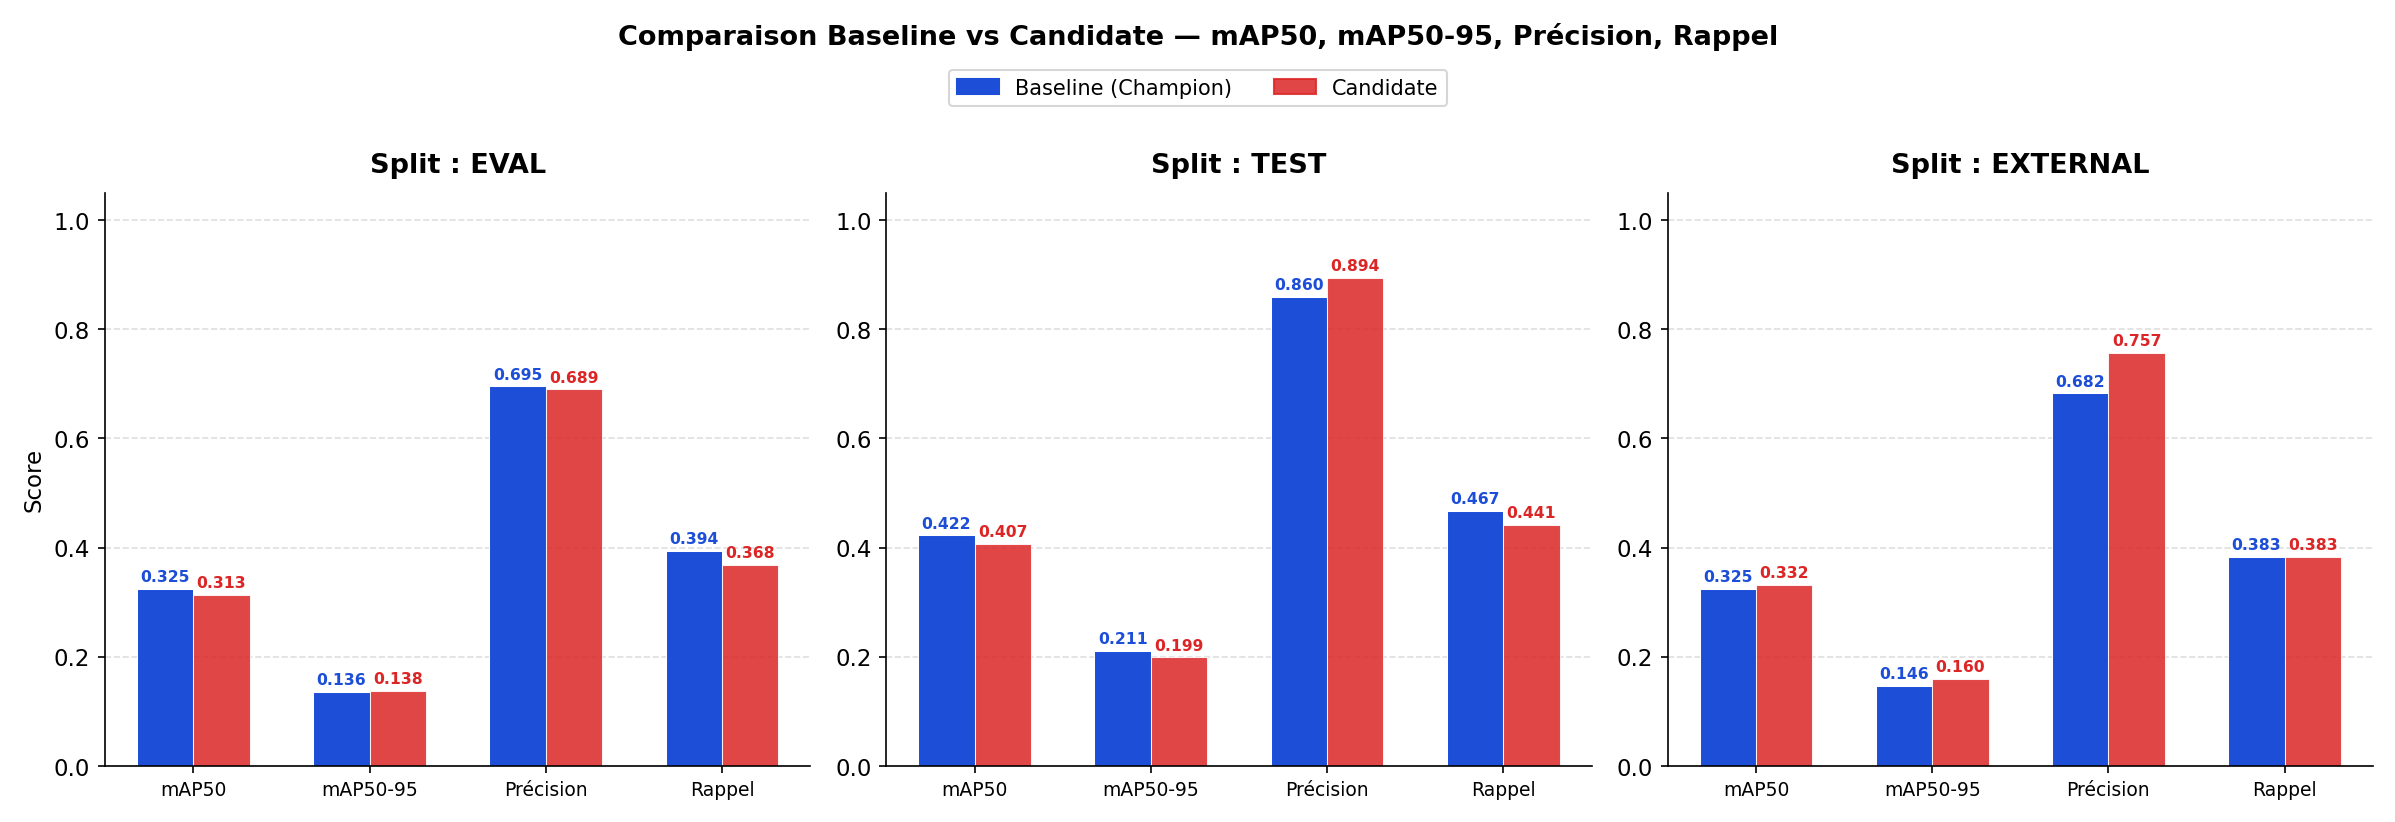
\includegraphics[width=\textwidth]{figures/eval_model_comparison.png}
\caption{Comparaison des performances Baseline vs Candidate sur les trois
         splits d'évaluation --- mAP50, mAP50-95, Précision et Rappel}
\label{fig:comparaison_modeles}
\end{figure}

\begin{figure}[H]
\centering
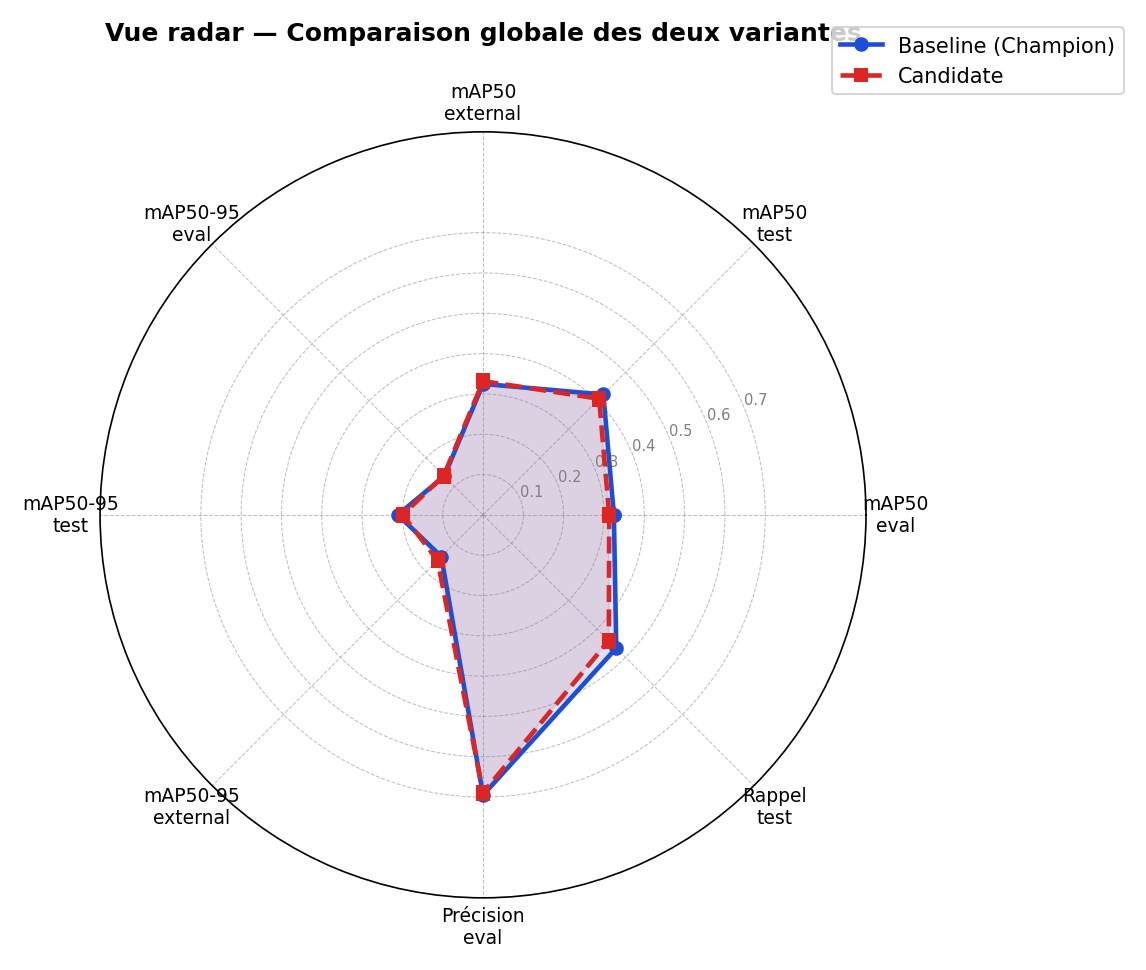
\includegraphics[width=0.78\textwidth]{figures/eval_model_radar.png}
\caption{Vue radar synthétique --- comparaison globale du modèle Champion
         (Baseline) et du Candidate sur 8 indicateurs de performance}
\label{fig:radar_modeles}
\end{figure}


\section{Registre de Modèles : Champion, Candidate, Archived}

\subsection{Principe du Registre}

Le projet implémente une logique de registre de modèles légère mais
rigoureuse, définie dans \projectpath{configs/model\_registry.yaml}.
Cette approche est une composante clé de la gouvernance MLOps : elle
formalise la décision de sélection, maintient un historique des modèles
promus et archivés, et découple le chemin du modèle en production
des chemins internes aux runs d'entraînement.

Trois rôles sont définis :
\begin{itemize}
    \item \textbf{Champion} : modèle sélectionné pour la production,
          exposé via l'alias stable
          \projectpath{models/checkpoints/champion/weights/best.pt} ;
    \item \textbf{Candidate} : modèle en cours d'évaluation comparative,
          potentiellement appelé à remplacer le Champion ;
    \item \textbf{Archived} : modèle retiré de la compétition, conservé
          pour la traçabilité historique.
\end{itemize}

\subsection{État Actuel du Registre}

L'état courant du registre, persisté dans
\projectpath{configs/model\_registry.yaml}, est le suivant :

\begin{table}[H]
\centering
\caption{État du registre de modèles du projet}
\label{tab:registre}
\begin{tabular}{p{2cm} p{5.5cm} p{6.5cm}}
\toprule
\textbf{Rôle} & \textbf{Modèle} & \textbf{Justification} \\
\midrule
\textbf{Champion}
  & \texttt{yolov8s\_7classes\_baseline}
    Run ID : \texttt{03fa528c...}
  & Meilleur compromis global sur eval et test, avec de bonnes
    performances sur external. Politique : \texttt{best\_global\_compromise} \\
\midrule
\textbf{Candidate}
  & \texttt{yolov8s\_7classes\_ext} \newline \texttt{ \_generalization\_v1}
     \newline Run ID : \texttt{dba1757b...}
  & Meilleur sur external ($+0.0132$ mAP50-95), mais moins bon
    en compromis global. Candidat pour une prochaine promotion. \\
\midrule
\textbf{Archived}
  & \texttt{yolov8s\_7classes\_v2} \newline \texttt{  \_small\_lesions}
  & Variante expérimentale ciblant les petites lésions. Compromis
    global inférieur aux deux autres variantes. Conservée pour
    la traçabilité. \\
\bottomrule
\end{tabular}
\end{table}

\subsection{Alias Stable du Champion}

Un mécanisme d'alias stable est implémenté pour découpler la
consommation du modèle Champion de son emplacement d'origine.
Lors de la promotion d'un checkpoint en Champion via le script
\projectpath{scripts/register\_best\_model.py}, le fichier
\texttt{best.pt} est copié vers :

\begin{center}
\texttt{models/checkpoints/champion/weights/best.pt}
\end{center}

Tous les composants en aval — script d'évaluation, service API,
configuration d'inférence — pointent vers cet alias  m.
Changer de modèle Champion ne nécessite donc qu'une seule commande :

\begin{verbatim}
python scripts/register_best_model.py \
    --checkpoint models/checkpoints/yolov8s_7classes_baseline/weights/best.pt \
    --role champion \
    --reason "meilleur compromis global sur eval et test"
\end{verbatim}

\subsection{Promotion et Archivage Automatiques}

Le script \projectpath{scripts/register\_best\_model.py} implémente
la logique complète de promotion :

\begin{enumerate}
    \item Lecture du registre courant depuis
          \projectpath{configs/model\_registry.yaml} ;
    \item Si le rôle demandé est Champion, l'ancien Champion est
          automatiquement archivé avant la promotion du nouveau ;
    \item Le checkpoint source est copié vers l'alias stable ;
    \item Le registre est mis à jour avec les nouvelles métadonnées
          (nom, checkpoint, rationale, source\_run\_id) ;
    \item Si un \texttt{run\_id} MLflow est fourni, les tags
          \texttt{selection\_role}, \texttt{selection\_reason} et
          \texttt{selected\_model\_name} sont ajoutés au run MLflow
          correspondant.
\end{enumerate}

\section{Décision de Sélection et Justification}

\subsection{Raisonnement MLOps}

La décision de sélectionner \texttt{yolov8s\_7classes\_baseline}
comme Champion repose sur une logique de \textbf{compromis global}
plutôt que sur l'optimisation d'une seule métrique ou d'un seul split.
Cette approche est fondamentale en MLOps : un modèle qui excelle
sur un seul contexte au détriment des autres est moins fiable
qu'un modèle qui performe de manière cohérente sur l'ensemble
des partitions.

\begin{table}[H]
\centering
\caption{Grille de décision multicritère pour la sélection du Champion}
\label{tab:decision_grille}
\begin{tabular}{p{4.5cm} cc p{4.5cm}}
\toprule
\textbf{Critère} & \textbf{Baseline} & \textbf{Candidate} & \textbf{Verdict} \\
\midrule
mAP50 sur eval         & \textbf{0.3246} & 0.3129 & Baseline +0.0117 \\
mAP50 sur test         & \textbf{0.4222} & 0.4072 & Baseline +0.0150 \\
mAP50 sur external     & 0.3248 & \textbf{0.3317} & Candidate +0.0069 \\
mAP50-95 sur eval      & 0.1358 & \textbf{0.1378} & Candidate +0.0020 \\
mAP50-95 sur test      & \textbf{0.2113} & 0.1992 & Baseline +0.0121 \\
mAP50-95 sur external  & 0.1464 & \textbf{0.1596} & Candidate +0.0132 \\
Rappel sur eval        & \textbf{0.3935} & 0.3679 & Baseline +0.0256 \\
Rappel sur test        & \textbf{0.4674} & 0.4412 & Baseline +0.0262 \\
\midrule
\textbf{Score global}  & \textbf{5/8} & 3/8 & \textbf{Baseline Champion} \\
\bottomrule
\end{tabular}
\end{table}

\subsection{Limites et Perspectives}

L'analyse des résultats met en évidence plusieurs axes d'amélioration
pour les travaux futurs.

\textbf{Rappel global faible.} Avec un rappel de 0.39 sur eval et
0.38 sur external, le modèle Champion manque environ 60\% des objets
présents. Cette limitation est partiellement liée au déséquilibre de
classes : les classes minoritaires comme \texttt{IMPACTED\_TOOTH}
et \texttt{PERIAPICAL\_PATHOLOGY} contribuent négativement au rappel global.

\textbf{Écart eval/test.} La différence de mAP50 entre eval (0.3246)
et test (0.4222) suggère une composition différente de ces deux splits.
Une analyse par classe des performances permettrait d'identifier
précisément quelles classes expliquent cet écart.

\textbf{Potentiel de la Candidate.} Le gain de $+0.0132$ en mAP50-95
sur external indique que la stratégie de la Candidate améliore la
précision géométrique des localisations sur données hors distribution.
Une variante combinant les forces des deux modèles constitue une
piste d'amélioration naturelle.

\section{Conclusion}

Ce chapitre a présenté l'évaluation complète et comparative des deux
variantes principales entraînées dans ce projet. Les résultats,
tous issus de fichiers JSON traçables et loggés dans MLflow,
établissent clairement la supériorité du Baseline en compromis
global avec un mAP50 de \textbf{0.3246} sur eval, \textbf{0.4222}
sur test et \textbf{0.3248} sur external. La décision de promotion
en Champion est formalisée dans le registre de modèles et exécutable
via une commande CLI reproductible. Les perspectives identifiées
— amélioration du rappel, analyse par classe, optimisation de la
généralisation externe — constituent des axes naturels de continuation
pour la phase suivante du projet.


\chapter{Déploiement et Industrialisation}
\label{chap:deployment}

\section{Introduction}

La sixième et dernière phase de CRISP-DM, le déploiement (\textit{Deployment}),
vise à rendre le modèle sélectionné accessible aux utilisateurs finaux dans
un environnement opérationnel. Dans un projet MLOps, cette phase ne se limite
pas à exporter un fichier de poids : elle englobe la conception d'une interface
d'accès standardisée, la conteneurisation du service pour assurer sa portabilité,
l'automatisation des vérifications via des pipelines CI/CD, et la mise à disposition
d'une interface de démonstration. Ce chapitre présente l'ensemble de ces composants
tels qu'ils ont été réalisés dans ce projet.

\section{Service d'Inférence REST avec FastAPI}

\subsection{Architecture du Service}

Le modèle Champion est exposé via un service HTTP construit avec
FastAPI~\cite{fastapi2019}. L'application est définie dans le module
\projectpath{src/detection\_dentaire/serving/api.py} et lancée par le
script \projectpath{scripts/serve\_api.py}.

L'architecture du service repose sur une classe centrale \texttt{PredictorService}
qui encapsule toute la logique de serving :

\begin{itemize}
    \item \textbf{Chargement paresseux} (\textit{lazy loading}) : le modèle
          YOLOv8 n'est instancié qu'à la première requête de prédiction,
          évitant un temps de démarrage long et permettant de vérifier
          rapidement la santé du service avant tout chargement GPU ;
    \item \textbf{Résolution de configuration} : le service charge
          \projectpath{configs/infer.yaml} au démarrage et résout
          automatiquement le chemin du checkpoint Champion via l'alias stable
          \projectpath{models/checkpoints/champion/weights/best.pt} ;
    \item \textbf{Gestion des uploads} : les images uploadées sont sauvegardées
          dans un fichier temporaire, traitées par le prédicteur, puis
          le fichier temporaire est supprimé dans un bloc \texttt{finally}
          pour éviter toute fuite de ressources.
\end{itemize}

\subsection{Endpoints de l'API}

\begin{table}[H]
\centering
\caption{Endpoints exposés par l'API REST}
\label{tab:api_endpoints}
\begin{tabular}{p{1.5cm} p{3cm} p{9.5cm}}
\toprule
\textbf{Méthode} & \textbf{Endpoint} & \textbf{Description} \\
\midrule
GET & \texttt{/}
  & Endpoint racine. Retourne un message de confirmation que le service
    est actif, avec les liens vers \texttt{/docs}, \texttt{/health}
    et \texttt{/predict}. \\
\midrule
GET & \texttt{/health}
  & Vérification de santé du service. Retourne le statut, le nom du modèle
    actif, le chemin du checkpoint, son existence sur disque et l'état
    de chargement du modèle en mémoire. \\
\midrule
GET & \texttt{/model-info}
  & Informations sur le modèle actif : nom, chemin du checkpoint,
    existence du fichier, chemin de configuration. \\
\midrule
POST & \texttt{/predict}
  & Endpoint principal d'inférence. Accepte une image en multipart/form-data
    et des paramètres optionnels (\texttt{image\_size}, \texttt{conf\_threshold},
    \texttt{iou\_threshold}, \texttt{max\_det}). Retourne un JSON structuré
    avec les détections. \\
\bottomrule
\end{tabular}
\end{table}

\subsection{Format de Réponse de \texttt{/predict}}

Le endpoint \texttt{POST /predict} retourne un objet JSON structuré contenant
toutes les informations nécessaires à une exploitation aval :

\begin{table}[H]
\centering
\caption{Structure de la réponse JSON du endpoint \texttt{/predict}}
\label{tab:api_response}
\begin{tabular}{p{3.5cm} p{2.5cm} p{8cm}}
\toprule
\textbf{Champ} & \textbf{Type} & \textbf{Description} \\
\midrule
\texttt{model\_name}       & string  & Nom du modèle Champion actif \\
\texttt{checkpoint\_path}  & string  & Chemin absolu du checkpoint utilisé \\
\texttt{image\_name}       & string  & Nom du fichier uploadé \\
\texttt{image\_width}      & integer & Largeur de l'image traitée (pixels) \\
\texttt{image\_height}     & integer & Hauteur de l'image traitée (pixels) \\
\texttt{num\_detections}   & integer & Nombre total d'objets détectés \\
\texttt{settings}          & object  & Paramètres d'inférence effectivement utilisés \\
\texttt{detections}        & array   & Liste des détections, triée par confiance \\
\midrule
\multicolumn{3}{l}{\textit{Chaque élément de \texttt{detections} contient :}} \\
\texttt{class\_id}         & integer & Identifiant numérique de la classe $\in \{0,\ldots,6\}$ \\
\texttt{class\_name}       & string  & Nom interprétable (ex: \texttt{CARIES}) \\
\texttt{confidence}        & float   & Score de confiance $\in [0, 1]$ \\
\texttt{bbox\_xyxy}        & array   & Coordonnées absolues $[x_1, y_1, x_2, y_2]$ en pixels \\
\bottomrule
\end{tabular}
\end{table}

\subsection{Configuration CORS et Documentation Automatique}

Le service est configuré avec un middleware CORS (\textit{Cross-Origin Resource
Sharing}) autorisant toutes les origines, ce qui permet au frontend React de
communiquer avec l'API sans restriction lors du développement local. FastAPI
génère automatiquement une documentation interactive Swagger accessible sur
\texttt{http://127.0.0.1:8000/docs}, permettant de tester tous les endpoints
directement depuis le navigateur.

\begin{figure}[H]
\centering
\fbox{\begin{minipage}[c][0.18\textheight][c]{0.88\linewidth}
\centering
\textbf{[Screenshot à insérer]}\\[0.5em]
\textit{Documentation Swagger de l'API FastAPI sur /docs}\\[0.5em]
Capture montrant les 4 endpoints avec leurs paramètres et le bouton Try it out.
\end{minipage}}
\caption{Documentation interactive Swagger générée automatiquement par FastAPI}
\label{fig:swagger_ui}
\end{figure}

\subsection{Lancement du Service}

```bash
pip install -r requirements-service.txt
python scripts/serve_api.py --host 127.0.0.1 --port 8000
Le script accepte trois arguments CLI : \texttt{--host}, \texttt{--port}
et \texttt{--config} (chemin vers la configuration d'inférence).

\section{Frontend de Démonstration React}

\subsection{Présentation}

Le dossier \projectpath{frontend/} contient une application React 19 + Vite 8
qui transforme le système de détection en démonstration interactive accessible
depuis un navigateur. Cette interface permet de valider visuellement le
comportement du modèle sans nécessiter d'outil externe.

\subsection{Fonctionnalités}

\begin{table}[H]
\centering
\caption{Fonctionnalités de l'interface React de démonstration}
\label{tab:frontend_features}
\begin{tabular}{p{4cm} p{10cm}}
\toprule
\textbf{Fonctionnalité} & \textbf{Description} \\
\midrule
Upload d'image
  & Glisser-déposer ou clic pour sélectionner une radiographie.
    Formats acceptés : JPG, PNG, BMP, TIFF, WEBP. \\
\midrule
Préprocessing client-side
  & L'image est redimensionnée à la taille cible et les ajustements de
    luminosité/contraste sont appliqués via un canvas HTML5 avant envoi
    au serveur. \\
\midrule
Contrôles d'inférence
  & Sliders configurables pour \texttt{image\_size} (640/896/1024~px),
    \texttt{conf\_threshold} (0.1--0.9), \texttt{iou\_threshold} (0.1--0.9),
    \texttt{max\_det} (1--500). \\
\midrule
Réglages image
  & Sliders de luminosité (70--140\%) et contraste (80--170\%)
    appliqués avant envoi pour adapter les radiographies
    sous-exposées ou surexposées. \\
\midrule
Visualisation des bbox
  & Les boîtes englobantes sont superposées sur l'image préprocessée
    avec le nom de la classe et le score de confiance. \\
\midrule
Synthèse des détections
  & Affichage du nombre de détections, de la répartition par classe
    et de la liste détaillée avec coordonnées et scores. \\
\midrule
Infos modèle
  & En-tête affichant le nom du modèle actif, le statut du checkpoint
    et l'URL de l'API utilisée. \\
\bottomrule
\end{tabular}
\end{table}

\subsection{Architecture Technique}

Le frontend communique avec le backend via un proxy Vite configuré dans
\projectpath{frontend/vite.config.js} : toutes les requêtes vers \texttt{/api}
sont redirigées vers \texttt{http://127.0.0.1:8000}.

La variable d'environnement \texttt{VITE\_API\_BASE\_URL} permet de surcharger
l'URL de l'API pour pointer vers un serveur distant lors d'un déploiement
en production.

\begin{figure}[H]
\centering
\fbox{\begin{minipage}[c][0.22\textheight][c]{0.88\linewidth}
\centering
\textbf{[Screenshot à insérer]}\\[0.5em]
\textit{Interface React avec une radiographie chargée et les bbox affichées}\\[0.5em]
Capture montrant l'upload, les contrôles, la visualisation des bbox colorées
et la synthèse des détections par classe.
\end{minipage}}
\caption{Interface de démonstration React avec visualisation des prédictions}
\label{fig:frontend_demo}
\end{figure}

\subsection{Lancement Local}

\begin{verbatim}
cd frontend
npm install
npm run dev
\end{verbatim}

L'interface est accessible sur \texttt{http://127.0.0.1:5173}.

\section{Conteneurisation avec Docker}

\subsection{Stratégie de Conteneurisation}

Le service d'inférence est packagé dans une image Docker~\cite{docker2014}
dédiée au mode CPU, définie dans \projectpath{Dockerfile}. Le choix d'une
image CPU uniquement est délibéré : il évite le téléchargement des dépendances
CUDA volumineuses dans l'image de service, réduisant sa taille et simplifiant
son déploiement sur des infrastructures sans GPU.

\subsection{Structure du Dockerfile}

\begin{table}[H]
\centering
\caption{Analyse du Dockerfile du service}
\label{tab:dockerfile}
\begin{tabular}{p{4cm} p{10cm}}
\toprule
\textbf{Instruction} & \textbf{Rôle} \\
\midrule
\texttt{FROM python:3.11-slim}
  & Image de base légère Python 3.11 sur Debian Slim \\
\texttt{ENV PYTHONDONTWRITEBYTECODE=1}
  & Désactive la génération de fichiers \texttt{.pyc} \\
\texttt{ENV PYTHONUNBUFFERED=1}
  & Logs en temps réel dans le conteneur \\
\texttt{COPY requirements-service.txt .}
  & Copie uniquement les dépendances minimales du service \\
\texttt{RUN pip install ...}
  & Installation avec timeout et retries pour la robustesse réseau \\
\texttt{COPY . .}
  & Copie le code source du projet \\
\texttt{EXPOSE 8000}
  & Déclare le port d'écoute \\
\texttt{CMD [...serve\_api.py]}
  & Commande de démarrage du service \\
\bottomrule
\end{tabular}
\end{table}

\subsection{Construction et Exécution}

\begin{verbatim}
# Construction de l'image
docker build -t dental-detection-api:latest .

# Exécution du conteneur
docker run --rm -p 8000:8000 dental-detection-api:latest

# Avec montage du checkpoint externe
docker run --rm -p 8000:8000 \
    -v /chemin/vers/models:/app/models \
    dental-detection-api:latest
\end{verbatim}

\textbf{Note importante :} pour une inférence réelle, le checkpoint Champion
(\projectpath{models/checkpoints/champion/weights/best.pt}) doit être présent
dans le conteneur, soit inclus lors du build, soit monté comme volume.

\section{Intégration Continue et Déploiement Continu (CI/CD)}

\subsection{Vue d'Ensemble}

Le projet intègre deux workflows GitHub Actions définis dans
\projectpath{.github/workflows/} :

\begin{itemize}
    \item \projectpath{ci.yml} : pipeline de vérification continue (CI) ;
    \item \projectpath{cd-service.yml} : pipeline de construction de l'image Docker (CD).
\end{itemize}

\subsection{Pipeline CI (\texttt{ci.yml})}

\begin{table}[H]
\centering
\caption{Étapes du pipeline CI GitHub Actions}
\label{tab:ci_pipeline}
\begin{tabular}{p{4cm} p{10cm}}
\toprule
\textbf{Étape} & \textbf{Description} \\
\midrule
Déclencheurs
  & Push sur \texttt{main}, \texttt{master}, \texttt{develop} ;
    toute Pull Request \\
\midrule
Checkout
  & Récupération du code source via \texttt{actions/checkout@v4} \\
\midrule
Setup Python
  & Installation de Python 3.11 via \texttt{actions/setup-python@v5} \\
\midrule
Install dependencies
  & \texttt{pip install -r requirements.txt \&\& pip install -e .} \\
\midrule
Run tests
  & \texttt{pytest -q} --- exécution de tous les tests unitaires \\
\midrule
Verify service CLI
  & \texttt{python scripts/serve\_api.py --help} \\
\midrule
Verify registry CLI
  & \texttt{python scripts/register\_best\_model.py --help} \\
\midrule
Verify evaluation CLI
  & \texttt{python scripts/evaluate.py --help} \\
\bottomrule
\end{tabular}
\end{table}

\subsection{Pipeline CD (\texttt{cd-service.yml})}

\begin{table}[H]
\centering
\caption{Étapes du pipeline CD --- Construction de l'image Docker}
\label{tab:cd_pipeline}
\begin{tabular}{p{4cm} p{10cm}}
\toprule
\textbf{Étape} & \textbf{Description} \\
\midrule
Déclencheurs
  & Push sur \texttt{main}/\texttt{master} avec modification de
    \texttt{Dockerfile}, \texttt{requirements-service.txt},
    \texttt{src/} ou \texttt{scripts/serve\_api.py} ;
    déclenchement manuel (\texttt{workflow\_dispatch}) \\
\midrule
Checkout
  & Récupération du code source \\
\midrule
Setup Docker Buildx
  & Configuration via \texttt{docker/setup-buildx-action@v3} \\
\midrule
Build service image
  & Construction de \texttt{dental-detection-api:latest}
    avec \texttt{push: false} (validation sans publication) \\
\bottomrule
\end{tabular}
\end{table}

\begin{figure}[H]
\centering
\fbox{\begin{minipage}[c][0.18\textheight][c]{0.88\linewidth}
\centering
\textbf{[Screenshot à insérer]}\\[0.5em]
\textit{Onglet Actions GitHub --- workflows CI et CD réussis}\\[0.5em]
Capture montrant les runs verts des deux workflows avec leurs étapes.
\end{minipage}}
\caption{Pipelines CI/CD GitHub Actions --- vérification continue et build Docker}
\label{fig:github_actions}
\end{figure}

\section{Vue d'Ensemble du Système Déployé}

\subsection{Flux d'Utilisation}

\begin{enumerate}
    \item Le praticien ouvre l'interface React (\texttt{http://127.0.0.1:5173}) ;
    \item Il uploade une radiographie panoramique par glisser-déposer ;
    \item Il configure optionnellement les seuils d'inférence et le préprocessing ;
    \item Le frontend redimensionne l'image et l'envoie via \texttt{POST /api/predict} ;
    \item Le service FastAPI analyse l'image via le modèle Champion et retourne le JSON ;
    \item Le frontend affiche les bbox avec classes et scores de confiance ;
    \item Le praticien consulte la synthèse des détections par classe.
\end{enumerate}

\section{Conclusion}

Ce chapitre a présenté l'ensemble de la phase de déploiement du projet.
L'API REST FastAPI expose le modèle Champion via une interface standardisée
et documentée automatiquement. Le frontend React offre une démonstration
interactive sans compétences techniques. L'image Docker garantit la portabilité
sur tout environnement. Les pipelines GitHub Actions automatisent la
vérification continue et la validation du packaging. Ensemble, ces composants
transforment un modèle expérimental en un système ML opérationnel conforme
aux exigences d'un projet d'ingénierie MLOps de niveau ingénieur.

% ============================================================
%  BIBLIOGRAPHIE
% ============================================================
\bibliographystyle{plain}
\bibliography{refs}

\end{document}